\documentclass[article]{jss}

%% -- LaTeX packages and custom commands ---------------------------------------

%% recommended packages
\usepackage{thumbpdf,lmodern}

%% another package (only for this demo article)
\usepackage{framed}

%% Packages from FCVAR.m
\usepackage{amsmath}
\usepackage{amsfonts}
\usepackage{float}   % used for better positioning of figures
\usepackage{mathrsfs} % for script fonts
% \usepackage[FIGTOPCAP]{subfigure}     %FIGTOPCAP puts captions on top of subfigures
\usepackage{subfigure}     %FIGTOPCAP puts captions on top of subfigures (not for JSS)
% \usepackage{subfig}

%% new custom commands
\newcommand{\class}[1]{`\code{#1}'}
\newcommand{\fct}[1]{\code{#1()}}

%% new custom commands from FCVAR.m
\def\lrt{{\rm LR}_T}


%% -- Article metainformation (author, title, ...) -----------------------------

%% - \author{} with primary affiliation
%% - \Plainauthor{} without affiliations
%% - Separate authors by \And or \AND (in \author) or by comma (in \Plainauthor).
%% - \AND starts a new line, \And does not.
\author{Lealand Morin\\University of Central Florida
   \And Morten \O rregaard Nielsen\\Queen's University and CREATES
   \AND Micha\l{} Ksawery Popiel\\Analysis Group}
\Plainauthor{Lealand Morin, Morten \O rregaard Nielsen, Micha\l{} Ksawery Popiel}

%% - \title{} in title case
%% - \Plaintitle{} without LaTeX markup (if any)
%% - \Shorttitle{} with LaTeX markup (if any), used as running title
\title{The Fractionally Cointegrated Vector Autoregression Model in \proglang{R}}
\Plaintitle{The Fractionally Cointegrated Vector Autoregression Model in R}
\Shorttitle{Fractionally Cointegrated VAR in \proglang{R}}

%% - \Abstract{} almost as usual
%% I figure that it is best to explain what this package does in plain English,  
%% in case any normal people get past the title and want to know what this package does. 
\Abstract{
  This article illustrates how to estimate 
  the fractionally cointegrated vector autoregression model (FCVAR) in \proglang{R}, based on a companion package in \proglang{MATLAB}. 
  This model is used to detect equilibrium relationships between variables observed over time. 
  The cointegrated vector autoregression model (CVAR) can detect an equilibrium relationship between variables that are integrated, i.e. exhibit unit root behavior, where deviations from this relationship are not integrated. 
  The fractionally cointegrated VAR model can detect relationships between variables that are cointegrated of a fractional order, with deviations that can be fractionally integrated but of a lower order than the variables themselves. 
  This allows for the detection of relationships with deviations that correct more slowly. 
The \pkg{FCVAR} package ties together the features of these models in a multivariate framework that allows for an exhaustive set of testing options. 




}

%% - \Keywords{} with LaTeX markup, at least one required
%% - \Plainkeywords{} without LaTeX markup (if necessary)
%% - Should be comma-separated and in sentence case.
\Keywords{cofractional process, cointegration rank, fractional autoregressive model, fractional cointegration, fractional unit root, \proglang{MATLAB}, \proglang{R}, VAR model}
\Plainkeywords{cofractional process, cointegration rank, fractional autoregressive model, fractional cointegration, fractional unit root, MATLAB, R, VAR model}

%% - \Address{} of at least one author
%% - May contain multiple affiliations for each author
%%   (in extra lines, separated by \emph{and}\\).
%% - May contain multiple authors for the same affiliation
%%   (in the same first line, separated by comma).
\Address{
  Morten \O rregaard Nielsen\\
  Queen's University\\
  Address \\
  \emph{and}\\
  CREATES\\
  Address \\
  E-mail: \email{mon@econ.queensu.ca}\\
  URL: \url{https://mortens.webpage/~software/}\\
  \phantom{0}\\
  Micha\l{} Ksawery Popiel\\
  Analysis Group\\
  E-mail: \email{Michal.Popiel@analysisgroup.com}\\
  \phantom{0}\\
  Lealand Morin\\
  Department of Economics\\
  University of Central Florida\\
  E-mail: \email{Lealand.Morin@ucf.edu}
}

\begin{document}


%% -- Introduction -------------------------------------------------------------

%% - In principle "as usual".
%% - But should typically have some discussion of both _software_ and _methods_.
%% - Use \proglang{}, \pkg{}, and \code{} markup throughout the manuscript.
%% - If such markup is in (sub)section titles, a plain text version has to be
%%   added as well.
%% - All software mentioned should be properly \cite-d.
%% - All abbreviations should be introduced.
%% - Unless the expansions of abbreviations are proper names (like "Journal
%%   of Statistical Software" above) they should be in sentence case (like
%%   "generalized linear models" below).

\section[Introduction: Cointegration and fractional integration in R]{Introduction: Cointegration and fractional integration in \proglang{R}} \label{sec:intro}

% JSS Notes:
%\begin{leftbar}
%The introduction is in principle ``as usual''. However, it should usually embed
%both the implemented \emph{methods} and the \emph{software} into the respective
%relevant literature. For the latter both competing and complementary software
%should be discussed (within the same software environment and beyond), bringing
%out relative (dis)advantages. All software mentioned should be properly
%\verb|\cite{}|d. 
% 
%For writing about software JSS requires authors to use the markup
%\verb|\proglang{}| (programming languages and large programmable systems),
%\verb|\pkg{}| (software packages), \verb|\code{}| (functions, commands,
%arguments, etc.). If there is such markup in (sub)section titles (as above), a
%plain text version has to be provided in the {\LaTeX} command as well. Below we
%also illustrate how abbrevations should be introduced and citation commands can
%be employed. See the {\LaTeX} code for more details.
% \end{leftbar}

This article illustrates how to estimate 
  the fractionally cointegrated vector autoregression model (FCVAR) in \proglang{R}. 
This model is used to detect equilibrium relationships between variables observed over time. 
The cointegrated vector autoregression model (CVAR) can detect an equilibrium relationship between variables that are integrated, i.e. exhibit unit root behavior, where deviations from this relationship are not integrated. 
The fractionally cointegrated VAR model can detect relationships between variables that are cointegrated of a fractional order, with deviations that can be fractionally integrated but of a lower order than the variables themselves. 
This allows for the detection of relationships with deviations that correct more slowly than with the CVAR. 
% 
The packages currently available concentrate more heavily on the features of one of these two types of models. 
% 

Existing software concentrates on either the CVAR alone, which is restricted to integer orders of integration, or focuses on specific features of the variables, such as estimating the integration order, identifying whether a  cointegrating relationship exists, or estimating a single-equation model.
Those that do consider fractionally cointegrated systems follow approaches developed earlier in the literature. 
The software in \pkg{FCVAR} treats the time series as a system and estimates all parameters together in a maximum likelihood framework and it provides a flexible set of options for conducting inference on many features of the cointegrating relationship. 

% 
An exhaustive listing of the R packages \citep{R} available for time series analysis were compiled in 
\citet{Hyndman2020}.
% \emph{CRAN Task View: Time Series Analysis} by Rob J Hyndman, 
% available at \verb|https://CRAN.R-project.org/view=TimeSeries|). 
% 
Among these, the packages most relevant to the FCVAR model are those related to cointegration within the family of vector error correction models or those related to long memory, often under the $ARFIMA$ framework. 

% \subsection{R packages for estimating the CVAR model}


In \proglang{R}, contegration analysis can be conducted using a variety of packages. 
% 
One such package is \pkg{aTSA} for \emph{Alternative Time Series Analysis} \citep{aTSA2015}. 
In this package, the \fct{coint.test} function performs Engle-Granger tests, as in \citet{EngleGranger1987},  for the null hypothesis that two or more time series, each of which is I(1), are not cointegrated. 
This package is designed to focus on a particular response variable, restricting attention to relationships with a one-dimensional cointegrating space. That is, this framework can detect a single equilibrium equation. 
% 
Another package following the \citet{EngleGranger1987} approach is the \pkg{egcm} package in \citep{egcm2017}. 
The \pkg{egcm} package restricts to a simplified form of cointegration. 
It is designed for bivariate analysis, with a concentration on applications to the prices of financial assets.

Other packages have implemeted the cointegration tests in \citet{PhillipsOuliaris1990}. 
This amounts to running a regression of the response variable on a set of regressors and testing the residuals for a unit root following \cite{PhillipsPerron1988}. 
The \fct{po.test} from the \pkg{tseries} package \citep{tseries2019} implements this test, 
as well as the \fct{ca.po} function in the \pkg{urca} package \citep{urca2016}. 

The \pkg{cointReg} package in \cite{cointReg2016} follows a different approach, using modified ordinary least squares (OLS) approaches to the analysis of cointegration. 
One such method is the fully modified OLS (FM-OLS) approach of \citet{PhillipsHansen1990} in the \fct{cointRegFM} function. 
Another option is the dynamic OLS (D-OLS) approach (see \citet{PhillipsLoretan1991}, \citet{Saikkonen1991} and \citet{StockWatson1993}) implemented in \fct{cointRegD}. 
It also implements, in \fct{cointRegIM}, a variant called integrated modified OLS (IM-OLS) of Vogelsang and Wagner (2014), 
which is based on an augmented integration transformation of the regression model. 

Following another approach, 
\citet{Johansen1995} analyzes the cointegrated VAR model in a more holistic fashion.
In this framework, the time series are treated as an endogenous system of equations and permits the estimation of a higher-dimensional cointegrating relationship, i.e. several equilibrium relationships. 
% 
It also allows for the joint estimation of parameters relating to the system of equations, permitting likelihood ratio tests for a wide variety of hypotheses. 
The \fct{VECM} function in the \pkg{tsDyn} package allows for the application of either the \citet{EngleGranger1987} or the \citet{Johansen1995} MLE method. 
However, this package is designed primarily with nonlinear time series models in mind. 
The \pkg{urca} package \citep{urca2016}, 
which is designed to perform unit root tests and cointegration analysis, 
follows the \citet{Johansen1995} approach in the function \fct{ca.jo}. 
It also provides options for testing restrictions on the parameters in the model. 
Of the packages designed for the CVAR model, this is perhaps the closest available to the \pkg{FCVAR} package, in terms of the testing opportunities available.

% \subsection{Segue from CVAR to $I(d)$}

While the packages that follow the framework of \citet{Johansen1995} are most closely related to the \pkg{FCVAR} package, these are not suited to the analysis of series with a fractional degree of integration. 
That is to say that these packages allow for only a discrete form of cointegration between the series. 
For example, the series are all integrated, i.e. $I(1)$, and the residuals from a regression are stationary and $I(0)$. 
The fractionally cointegrated VAR model allows for the possibility that variables can be integrated of order $d$ and cointegrated of order $d - b$, where $d$ and $b>0$ can be real numbers. 
% 
Analysis using the above packages typically involves a preliminary analysis of the form of non-stationarity of the variables, using a number of unit root tests, i.e. to test whether the series are $I(1)$. 
With fractionally integrated variables, the first stage of the analysis is to determine the order of fractional integration, i.e. the parameter $d$. 
This has been the focus of much of the available software to analyze series with the characteristics of so-called long memory. 

% \subsection{R packages for fractional integration}

In another section of the \emph{CRAN Task View: Time Series Analysis} \citep{Hyndman2020}, 
several packages are listed for the estimation of models for series with features of fractional integration or long memory. 
A number of these pacakages are focused on estimation of $ARFIMA$ models, known as autoregressive fractionally integrated moving average models. 
The \pkg{fracdiff} package \citep{fracdiff2020} includes functions for fitting $ARFIMA(p,d,q)$ models, including the step of estimating the long memory parameter $d$. 
The namesake function \fct{fracdiff} calculates the maximum likelihood estimators of the parameters of a fractionally-differenced $ARIMA(p,d,q)$ model. 
A few notable functions in this package estimate the long memory parameter $d$ within this model\footnote{Note that the \fct{diffseries} function in \pkg{fracdiff} is based on the same algorithm in \cite{Jensen2014} as \fct{FracDiff} in \pkg{FCVAR}, except that \fct{diffseries} demeans the data first. Specifically, \code{fracdiff::diffseries(x, d) - FCVAR::FracDiff(x - mean(x), d)} is numerically very small. 
The demeaning step is not required to estimate the FCVAR model, as the mean parameters are estimated jointly with the others while optimizing the likelihood function. }. 
% 
The \pkg{arfima} package \cite{arfima2018} fits a wider variety of $ARFIMA$ models. 
% 
Also, the \pkg{nsarfima} \citep{nsarfima2019} package provides methods for fitting and simulating non-stationary $ARFIMA$ models. 
This package is more innovative in terms of the types of optimization problems built on the $ARFIMA$ model, including both maximum likelihood (as in \citet{Beran1995}) and minimum distance (as in \citet{Mayoral2007}) estimators. 
Overall, $ARFIMA$ models treat the data by fractional differencing to transform data to a form suitable for an $ARMA$ model, 
similar to ordinary first differencing for variables that have unit roots as in $ARIMA$ models. 
This transformation precludes the use of models that study cointegration relationships. 

The package \pkg{LongMemoryTS} is in a class of its own, in that it uses a wide variety of methods to investigate both fractional integration and cointegrating relationships.\footnote{Morten: You would be best suited to comment on the references in this package. 
There are several citations to your papers and papers that I'm sure you know better and I want to make sure that we are honest about the difference between what we do and what they do. 
It seems to me that this package is a who's who of analyzing the cointegration of fractional systems, except for Johansen's MLE framework, which is what we implement.
I like to think that our approach following \citet{Johansen1995} is more holistic, in that all the parameters are estimated jointly, aside from the rank and lag selection. 
It captures all of the pieces in one maximum likelihood framework and this approach has the added benefit of allowing for a wide range of restrictions to test. 

\textbf{Before I forget}, one important point to note is that I did not succeed in installing this package. 
It requires dependencies that would not install on either my local machine or the ones in Dunning 211 or the equivalent at UCF. 
I'm a patient guy but f I can't get it to work in 10 minutes, their user base is going to be very small. 
That's too bad, because they have also implemented \cite{Jensen2014}, with your permission, in the function \fct{fdiff}. I would have liked to test it for myself. 
In my opinion, they have too much going on in one package and the level of complexity can lead to dependency problems like this. 
As a user, I would move on to the next package that works, which is a good reason to implement this function ourselves, without these problems. 
Actually, now that I have looked at it more closely, the documentation is incomplete as well. 
Our closest competitor is a work in progress -- but there is no need to call them out on it. } 
% 
For estimating the order of the fractional integration in a series, there are several options including the log-periodogram estimators of \citet{GPH1983} and \citet{RobinsonPM1995b}. 
% 
Other options include the semiparametric local Whittle estimator of \citet{RobinsonPM1995a},
the exact local Whittle estimator of \citet{ShimotsuPhillips2005}, 
and a version for series with unknown mean and time trend in \citet{Shimotsu2010}. 
They also implement more recent approaches, such as 
the local polynomial Whittle plus noise estimator of \citet{FredNielsenNielsen2012} 
and the modified local Whittle estimator of \citet{HouPerron2014}. 


For determining the cointegrating rank, i.e. the dimension of the cointegrating relationship, this package also provides several options. 
These inclide a semiparametric method in \citet{ChenHurvich2003}. 
\citet{RobinsonYajima2002} propose a model selection procedure to estimate the cointegrating rank ,
which includes a test for equality of all memory parameters simultaneously and is further explored in \citet{NielsenShimotsu2007}. 
Following another approach, the package also provides a method of
identifying cointegration by eigenanalysis \citep{ZhangRobinsonYao2018}. 


Finally, for estimation the cointegrating relationship itself, the \pkg{LongMemoryTS} package implements a number of approaches. 
It implements semiparametric approaches for estimating the cointegrating vector, including that of 
\citet{Robinson1994} and later \citet{RobinsonMarinucci2003} and \citet{ChristensenNielsen2006}. 
They implement a semiparametric residual-based test for fractional cointegration from \citet{ChenHurvich2006}, 
and other semiparametric tests in \citet{MarmolVelasco2004}and \citet{WangWangChan2015}
and a semiparametric Hausmann-type test for fractional cointegration by \citet{Robinson2008}. 
Also within the semiparametric family is the fully modified narrow band least squares (FMNBLS) approach in  \citet{NielsenFrederiksen2011}. 
% 
They also implement a nonparametric approach to test for fractional cointegration and rank estimation by \citet{Nielsen2010}.
Following another framework, the frequency-domain test for fractional cointegration in \citet{SouzaEtal2018} is also available in this package. 

In contrast, our approach is to use a fully parametric model in the maximum likelihood framework. 
The \pkg{FCVAR} package, introduced here, is closest to a cross between the \citet{Johansen1995} cointegration model in \pkg{urca} and the models involving fractionally integrated variables discussed above. 
In particular, the model estimated in the \pkg{urca} packages is the special case of \pkg{FCVAR} in which the fractional integration parameters $d$ and $b$ are both equal to one.\footnote{They also use the Danish data, so it might be worthwhile to include in the documentation an example with and without the restriction $d = b = 1$ to compare. It may not fit in this paper but could be a short vignette (short pdf with code and descriptions) that would go on the CRAN webpage for the package. } 
% 
% 
% \subsection{The  MATLAB program}
% 
The \proglang{R} package \pkg{FCVAR} closely follows a companion package \pkg{FCVARmodel.m}, written in \proglang{MATLAB}. 
The \proglang{MATLAB} package is documented in \cite{Nielsen2016}, an expanded version of the package documented in \cite{Nielsen2013}. 

% Moved to end, as per JSS style:
%The latest version of the package can be downloaded from one of the author's website at Queen's University:
%% 
%\begin{center} \url{http://www.econ.queensu.ca/faculty/mon/software/}
%\end{center}
%% 
%\noindent It is freely available for non-commercial, academic use. 
%The use of this program requires a functioning installation of MATLAB. 
%The version of \proglang{MATLAB} available at the release of the last version was \proglang{MATLAB} 9.0, 	R2016a, number 35. However, any recent version should work.  
%\proglang{MATLAB} users can simply unzip the contents of the zip file into any directory that they plan to use as the working directory of the program.

% \subsection{Roadmap}

The next section describes the FCVAR model and the restricted models that can be estimated with this program. Section \ref{sec:main} describes an example of a modeling session, which is a replication of one of the tables of results in \cite{JNP2014}. Section \ref{sec:examples} describes another example program, which demonstrates some additional functionality of the software. Importantly, these are the only two files that would need to be changed to apply the program for other empirical analyses. 
% Section \ref{sec programs} describes how each of the major program files work (each in a separate subsection). 
% The Appendix contains a version change log.
% These are removed as they belong in the package documentation. 

% JSS Style Notes:
%% -- Manuscript ---------------------------------------------------------------
%% - In principle "as usual" again.
%% - When using equations (e.g., {equation}, {eqnarray}, {align}, etc.
%%   avoid empty lines before and after the equation (which would signal a new
%%   paragraph.
%% - When describing longer chunks of code that are _not_ meant for execution
%%   (e.g., a function synopsis or list of arguments), the environment {Code}
%%   is recommended. Alternatively, a plain {verbatim} can also be used.
%%   (For executed code see the next section.)

% \section{Models and software} \label{sec:models}
\section{The fractionally cointegrated VAR model} \label{sec:fcvar}

% JSS notes:
%\begin{leftbar}
%Note that around the \verb|{equation}| above there should be no spaces (avoided
%in the {\LaTeX} code by \verb|%| lines) so that ``normal'' spacing is used and
%not a new paragraph started.
%\end{leftbar}

The fractionally cointegrated vector autoregressive (FCVAR) model was proposed in \cite{Johansen2008} and analyzed by, e.g., \cite{johniel2010,johansen2012likelihood}. For a time series $X_{t}$ of dimension $p$, the fractionally cointegrated VAR model is given in error correction form as
\begin{equation}
\Delta^{d}X_{t}= \alpha \beta^{\prime} \Delta^{d-b} L_{b} X_{t} + 
\sum_{i=1}^{k}\Gamma_{i}\Delta^{d}\ L_{b}^{i}X_{t}
+ \varepsilon_{t},
\label{vecm model}%
\end{equation}
where $\varepsilon_{t}$ is $p$-dimensional $i.i.d.(0,\Omega)$, $\Delta^{d}$ is the fractional difference operator, and $L_{b}=1-\Delta^{b}$ is the fractional lag operator.\footnote{Both the fractional difference and fractional lag operators are defined in terms of their binomial expansion in the lag operator, $L$. Note that the expansion of $L_{b}$ has no term in $L^{0}$ and thus only lagged disequilibrium errors appear in \eqref{vecm model}.} \cite{johansen2012likelihood} imposed two restrictions on the parameter space, $d\geq b$ and $d-b<1/2$, in their asymptotic analysis. However, these restrictions were relaxed in \cite{JN2018b,JN2018}.

Model \eqref{vecm model} includes the \cite{Johansen1995} CVAR model as the special case $d=b=1$; see \cite{JN2018}. Some of the parameters are well-known from the CVAR model and these have the usual interpretations also in the FCVAR model. The most important of these are the long-run parameters $\alpha$ and $\beta$, which are $p \times r$ matrices with $0 \leq r \leq p$. The rank $r$ is termed the cointegration, or cofractional, rank. The columns of $\beta$ constitute the $r$ cointegration (cofractional) vectors such that $\beta' X_t$ are the cointegrating combinations of the variables in the system, i.e.\ the long-run equilibrium relations. The parameters in $\alpha$ are the adjustment or loading coefficients which represent the speed of adjustment towards equilibrium for each of the variables. The short-run dynamics of the variables are governed by the parameters $\Gamma=(\Gamma _{1},\ldots ,\Gamma _{k})$ in the autoregressive augmentation.

The FCVAR model has two additional parameters compared with the CVAR model, namely the fractional parameters $d$ and $b$. Here, $d$ denotes the fractional integration order of the observable time series and $b$ determines the degree of fractional cointegration, i.e.\ the reduction in fractional integration order of $\beta'X_t$ compared to $X_t$ itself. These parameters are estimated jointly with the remaining parameters. This model thus has the same main structure as in the standard CVAR model in that it allows for modeling of both cointegration and adjustment towards equilibrium, but is more general since it accommodates fractional integration and cointegration.

In the next four subsections we briefly describe the accommodation of deterministic terms as well as estimation and testing in the FCVAR model.

\subsection{Deterministic terms}

There are several ways to accommodate deterministic terms in the FCVAR model \eqref{vecm model}. The inclusion of the so-called restricted constant was considered in \cite{johansen2012likelihood}, and the so-called unrestricted constant term was considered in \cite{Dolatabadi2014}. A general formulation that encompasses both models is\footnote{In \cite{Dolatabadi2014} the constants are included as $\rho' \pi_t(1)$ and $\xi \pi_t(1)$, where $\pi_t(u)$ denotes coefficients in the binomial expansion of $(1-z)^{-u}$. This is mathematically convenient, but makes no difference in terms of the practical implementation.}
\begin{equation}
\Delta^{d}X_{t}= \alpha \Delta^{d-b} L_{b} (\beta^{\prime} X_{t} +\rho^{\prime}) + 
\sum_{i=1}^{k}\Gamma_{i}\Delta^{d}\ L_{b}^{i}X_{t} +\xi
+ \varepsilon_{t}.
\label{model with constants}
\end{equation}
The parameter $\rho $ is the so-called restricted constant term (since the constant term in the model is restricted to be of the form $\alpha \rho ^{\prime }$), which is interpreted as the mean level of the long-run equilibria when these are stationary, i.e.\ $E\beta ^{\prime }X_{t}+\rho ^{\prime }=0$. The parameter $\xi$ is the unrestricted constant term, which gives rise to a deterministic trend in the levels of the variables. When $d=1$ this trend is linear. Thus, the model \eqref{model with constants} contains both a restricted constant and an unrestricted constant. In the usual CVAR model, i.e.\ with $d=b=1$, the former would be absorbed in the latter, but in the fractional model they can both be present and are interpreted differently. For the representation theory related to \eqref{model with constants}, and in particular for additional interpretation of the two types of constant terms, see \cite{Dolatabadi2014}.

An alternative formulation of deterministic terms was suggested by \cite{johansen2014initial}, albeit in a simpler model, with the aim of reducing the impact of pre-sample observations of the process. This model is
\begin{equation}
\Delta^{d}(X_{t}-\mu)= \alpha \beta^{\prime} \Delta^{d-b} L_{b} (X_{t}-\mu) + 
\sum_{i=1}^{k}\Gamma_{i}\Delta^{d}\ L_{b}^{i}(X_{t}-\mu)
+ \varepsilon_{t},
\label{model with level par}
\end{equation}
which can be derived easily from the unobserved components formulation
\begin{equation}
X_t = \mu + X_t^0, \; \; \;
\Delta^{d}X_{t}^0=L_{b} \alpha \beta^{\prime} X_{t}^0 + 
\sum_{i=1}^{k}\Gamma_{i}\Delta^{d}\ L_{b}^{i}X_{t}^0
+ \varepsilon_{t}.
\label{UC model with level par}
\end{equation}
The formulation \eqref{model with level par}, or equivalently \eqref{UC model with level par}, includes the restricted constant, which may be obtained as $\rho'=\beta'\mu$. More generally, the level parameter $\mu$ is meant to accommodate a non-zero starting point for the first observation on the process, i.e., for $X_1$. It has the added advantage of reducing the bias arising due to pre-sample behavior of $X_t$, at least in simple models, even when conditioning on no initial values (see below). For details, see \cite{johansen2014initial}.


\subsection{Maximum likelihood estimation}

It is assumed that a sample of length $T+N$ is available on $X_t$, where $N$ denotes the number of observations used for conditioning, for details see \cite{johansen2014initial}. The models \eqref{vecm model}, \eqref{model with constants}, and \eqref{model with level par} are estimated by conditional maximum likelihood, conditional on $N$ initial values, by maximizing the function
\begin{equation}
\log L_{T}(\lambda ) = - \frac{T p}{2} ( \log(2\pi) + 1) 
-\frac{T}{2}\log \det \left\{ T^{-1}\sum_{t=N+1}^{T+N}\varepsilon _{t}(\lambda )\varepsilon _{t}(\lambda)^{\prime }\right\},  \label{Cond Like}
\end{equation}
where the residuals are defined as
\begin{equation}
\varepsilon _{t}(\lambda ) = \Delta^{d}X_{t}- \alpha \Delta^{d-b} L_{b} (\beta^{\prime} X_{t} + \rho') 
 - \sum_{i=1}^{k}\Gamma_{i}\Delta^{d}\ L_{b}^{i}X_{t} - \xi, \quad
\lambda =(d,b,\alpha,\beta,\Gamma,\rho,\xi),
\label{epstau}
\end{equation}
for model \eqref{model with constants}, and hence also for submodels of model \eqref{model with constants}, such as \eqref{vecm model}, with the appropriate restrictions imposed on $\rho$ and $\xi$. For model \eqref{model with level par} the residuals are
\begin{equation}
\varepsilon _{t}(\lambda ) = \Delta^{d}(X_{t}-\mu) -  \alpha \beta^{\prime} \Delta^{d-b} L_{b} (X_{t} - \mu) 
 - \sum_{i=1}^{k}\Gamma_{i}\Delta^{d}\ L_{b}^{i}(X_{t} - \mu), \quad
\lambda =(d,b,\alpha,\beta,\Gamma,\mu).
\label{epstau level}
\end{equation}
It is shown in \cite{johansen2012likelihood} and \cite{Dolatabadi2014} how, for fixed $(d,b)$, the estimation of model \eqref{model with constants} reduces to regression and reduced rank regression as in \cite{Johansen1995}. In this way the parameters $(\alpha ,\beta,\Gamma,\rho,\xi)$ can be concentrated out of the likelihood function, and numerical optimization is only needed to optimize the profile likelihood function over the two fractional parameters, $d$ and $b$. In model \eqref{model with level par} we can similarly concentrate the parameters $(\alpha ,\beta,\Gamma)$ out of the likelihood function resulting in numerical optimization over $(d,b,\mu)$, making the estimation of model \eqref{model with level par} slightly more involved numerically than that of model \eqref{model with constants}.

For model \eqref{model with constants} with $\xi=0$, \cite{johansen2012likelihood} shows that asymptotic theory is standard when $b<0.5$, and for the case $b>0.5$ asymptotic theory is non-standard and involves fractional Brownian motion of type II. Specifically, when $b>0.5$, \cite{johansen2012likelihood} shows that under i.i.d.\ errors with suitable moment conditions, the conditional maximum likelihood parameter estimates  $(\hat{d},\hat{b},\hat{\alpha},\hat{\Gamma}_{1},\ldots,\hat{\Gamma}_{k})$ are asymptotically Gaussian, while $(\hat{\beta},\hat{\rho})$\ are locally asymptotically mixed normal. These results allow asymptotically standard (chi-squared) inference on all parameters of the model, including the cointegrating relations and orders of fractionality, using quasi-likelihood ratio tests. As in the CVAR model, see \cite{Johansen1995}, the same results hold for the same parameters in the full models \eqref{model with constants} and \eqref{model with level par}, whereas the asymptotic distribution theory for the remaining parameters, $\xi$ and $\mu$, is currently unknown.


\subsection{Cointegration rank tests}

Letting $\Pi = \alpha \beta'$, the likelihood ratio (LR) test statistic of the hypothesis $\mathcal{H}_{r}: \mathrm{rank}(\Pi )=r$ against $\mathcal{H}_{p}:\mathrm{rank}(\Pi )=p$ is of particular interest because it deals with an important empirical question. This statistic is often denoted the ``trace'' statistic. Let $\theta = (d,b)$ for model \eqref{model with constants} and $\theta = (d,b,\mu)$ for model \eqref{model with level par} denote the parameters for which the likelihood is numerically maximized. Then let $L(\theta,r)$ be the profile likelihood function given rank $r$, where $(\alpha ,\beta ,\Gamma )$, and possibly $(\rho,\xi)$ if appropriate, have been concentrated out by regression and reduced rank regression; see \cite{johansen2012likelihood} and \cite{Dolatabadi2014} for details.

The profile likelihood function is maximized both under the hypothesis $\mathcal{H}_{r}$ and under $\mathcal{H}_{p}$ and the LR test statistic is then $\lrt(q)=2\log(L(\hat{\theta}_{p},p)/L(\hat{\theta}_{r},r))$, where 
\begin{equation*}
L(\hat{\theta}_{p},p)=\max_{\theta}L(\theta,p), \quad L(\hat{\theta}_{r},r)=\max_{\theta}L(\theta,r),
\end{equation*}
and $q=p-r$. This problem is qualitatively different from that in \cite{Johansen1995} since the asymptotic distribution of $\lrt(q)$ depends qualitatively (and quantitatively) on the parameter $b$. In the case with $0<b<1/2$ (sometimes known as \textquotedblleft weak cointegration\textquotedblright ), $\lrt(q)$ has a standard asymptotic distribution, see \citet[Theorem 11(ii)]{johansen2012likelihood}, namely 
\begin{equation}
\lrt(q)\overset{D}{\rightarrow }\chi ^{2}(q^{2}), \; \; 0<b<1/2.
\end{equation}
On the other hand, when $1/2<b\leq d$ (\textquotedblleft strong cointegration\textquotedblright ), asymptotic theory is nonstandard and 
\begin{equation}
\lrt(q)\overset{D}{\rightarrow }\mathrm{Tr}\left\{
\int_{0}^{1}\mathsf{d}W(s)F(s)^{\prime }\left( \int_{0}^{1}F(s)F(s)^{\prime}\mathsf{d}s\right) ^{-1}
\int_{0}^{1}F(s)\mathsf{d}W(s)^{\prime }\right\}, \; \; b>1/2,
\label{LR asy distr}
\end{equation}
where the vector process $\mathsf{d}W$ is the increment of ordinary (non-fractional) vector standard Brownian motion of dimension $q=p-r$. The vector process $F$ depends on the deterministics in a similar way as in the CVAR model in \cite{Johansen1995}, although the fractional orders complicate matters. The following cases have been derived in the literature:

 \begin{enumerate}
 \item When no deterministic term is in the model, $F(u)=W_{b}(u)$, where $W_{b}(u)=\Gamma(b)^{-1}\int_{0}^{u}(u-s)^{b-1}\mathsf{d}W(s)$ is vector fractional Brownian motion of type II, see \citet[Theorem 11(i)]{johansen2012likelihood}.
 \item When only the restricted constant term is included in model \eqref{model with constants}, $F(u)=(W_{b}(u)^{\prime},u^{-(d-b)})^{\prime }$, see \citet[Theorem 11(iv)]{johansen2012likelihood} for the result with $d=b$ and an earlier working paper version for the general result.
\item In model \eqref{model with level par} the same result as in bullet 2.\ holds because $\beta'\mu = \rho'$ is the restricted constant and $\beta_\perp^{\prime} \mu$ has no influence on the asymptotic distribution (in a similar way to $X_0$ in a random walk).
 \item When both the restricted and unrestricted constants are included in model \eqref{model with constants} with $d=1$,
\begin{align*}
F_{i}(u) &= W_{b,i}(u) - \int_{0}^{1} W_{b,i}(u) \mathsf{d} u, \ i=1,...,q-1, \\
F_{q}(u) &= u^{b} - \int_{0}^{1}u^{b} \mathsf{d} u=u^{b}-1/(b+1), \\
F_{q+1}(u) &= u^{b-1} - \int_{0}^{1}u^{b-1} \mathsf{d} u = u^{b-1}-1/b, 
\end{align*}
see \cite{Dolatabadi2014}.
\end{enumerate}

Importantly, the asymptotic distribution \eqref{LR asy distr} of the test statistic $\lrt(q)$ depends on both $b$ and $q=p-r$. The dependence on the unknown (true value of the) scalar parameter $b$ complicates empirical analysis compared to the CVAR model. Generally, the distribution \eqref{LR asy distr} would need to be simulated on a case-by-case basis. However, for model \eqref{vecm model} and for model \eqref{model with constants} with $d=b$ and $\xi=0$, and hence also for model \eqref{model with level par} with $d=b$ in light of bullet 3.\ above, computer programs for computing asymptotic critical values and asymptotic $P$ values for the LR cointegration rank tests based on numerical distribution functions, are made available by \cite{mackinnon2014numerical}. Their computer programs are incorporated in the present program for the relevant cases/models as discussed and illustrated below.



\subsection{Restricted models}
\label{restricted models}

Note that a reduced rank restriction has already been imposed on models \eqref{vecm model}--\eqref{model with level par}, where the coefficient matrix $\Pi  = \alpha \beta '$ has been restricted to rank $r \leq p$. Other restrictions on the model parameters can be considered as in \cite{Johansen1995}. The most interesting restrictions from an economic theory point of view would likely be restrictions on the adjustment parameters $\alpha$ and cointegration vectors $\beta$.

We formulate hypotheses as
\begin{align}
  &R_{\psi} \psi = r_{\psi}, \label{R psi} \\
  &R_\alpha \mathrm{vec}(\alpha) = 0, \label{R alpha} \\
  &R_\beta \mathrm{vec}(\beta^{\ast}) = r_\beta, \label{R beta}
\end{align}
with $\beta^{\ast} = (\beta', \rho')'$, and use the switching algorithm in \cite[p.\ 455]{Boswijk2004} to optimize the likelihood numerically subject to the restrictions. The switching algorithm can be improved by adding a line search, see \cite{Doornik2016}. This is done by setting the option \verb|opt$LineSearch = 1|, which is the default setting.

The only limitation on the linear restrictions that can be imposed on $(d,b,\alpha,\beta^{\ast})$ in \eqref{R psi}--\eqref{R beta} is that only homogenous restrictions can be imposed on $\mathrm{vec}(\alpha)$ in \eqref{R alpha}. Otherwise, any combination of linear restrictions can be imposed on these parameters. For now, the remaining parameters cannot be restricted.

Note that, when the restricted constant term $\rho$ is included in the model, restrictions on $\beta$ and $\rho$ must be written in the form given by \eqref{R beta}. This is without loss of generality.

The restrictions in \eqref{R psi}--\eqref{R beta} above can be implemented individually or simultaneously in the MATLAB program. The next section provides an example session illustrating the use of the program with a step-by-step description of a typical empirical analysis, including several restricted models in Section \ref{subsec hypo}.

\subsection{Forecasting from the FCVAR model}

Because the FCVAR model is autoregressive, the best linear predictor takes a simple form and is relatively straightforward to calculate. Consider, for example, the model with level parameter in \eqref{model with level par}. We first note that
\begin{equation}
\Delta^d (X_{t+1}-\mu) = X_{t+1}-\mu  - (X_{t+1}-\mu) + \Delta^d (X_{t+1}-\mu) = X_{t+1}-\mu - L_d (X_{t+1}-\mu)
\nonumber
\end{equation}
and then rearrange (\ref{model with level par}) as
\begin{equation}
X_{t+1}=\mu + L_d (X_{t+1}-\mu)+\alpha\beta^{\prime}\Delta^{d-b}L_{b}(X_{t+1}-\mu)+\sum
_{i=1}^{k}\Gamma_{i}\Delta^d L_{b}^{i}(X_{t+1}-\mu)+\varepsilon_{t+1}.
\label{model forecast}
\end{equation}
Since $L_{b}=1-\Delta^{b}$ is a lag operator, so that $L_{b}^{i}X_{t+1}$ is known at time $t$ for $i \geq 1$, this equation can be used as the basis to calculate forecasts from the model.

We let conditional expectation given the information set at time $t$ be denoted $E_{t}(\cdot)$, and the best linear predictor forecast of any variable $Z_{t+1}$ given information available at time $t$ be denoted $\hat{Z}_{t+1|t}=E_{t}(Z_{t+1})$. Clearly, we then have that the forecast of the innovation for period $t+1$ at time $t$ is $\hat{\varepsilon}_{t+1|t}=E_{t}(\varepsilon_{t+1})=0$, and $\hat{X}_{t+1|t}$ is then easily found from (\ref{model forecast}). Inserting also coefficient estimates based on data available up to time $t$, denoted\footnote{To emphasize that these estimates are based on data available at time $t$, they could be denoted by a subscript $t$. However, to avoid cluttering the notation we omit this subscript and let it be understood in the sequel.} $(\hat{d},\hat{b},\hat{\mu},\hat{\alpha},\hat{\beta },\hat{\Gamma}_{1},\ldots,\hat{\Gamma}_{k})$, we have that
\begin{equation}
\hat{X}_{t+1|t}=\hat{\mu}+L_{\hat{d}} (X_{t+1}-\hat{\mu})+\hat{\alpha}\hat{\beta}^{\prime}\Delta^{\hat{d}-\hat{b}
}L_{\hat{b}}(X_{t+1}-\hat{\mu})+\sum_{i=1}^{k}\hat{\Gamma}_{i}\Delta^{\hat{d}}
L_{\hat{b}}^{i}(X_{t+1}-\hat{\mu}).
\label{forecast one}
\end{equation}
This defines the one-step ahead forecast of $X_{t+1}$ given information at time $t$. 

Multi-period ahead forecasts can be generated recursively. That is, to calculate the $h$-step ahead forecast, we first generalize (\ref{forecast one}) as
\begin{equation}
\hat{X}_{t+j|t}=\hat{\mu}+L_{\hat{d}} (\hat{X}_{t+j|t}-\hat{\mu})+\hat{\alpha}\hat{\beta}^{\prime}
\Delta^{\hat{d}-\hat{b}}L_{\hat{b}}(\hat{X}_{t+j|t}-\hat{\mu})+\sum_{i=1}^{k}
\hat{\Gamma}_{i}\Delta^{\hat{d}} L_{\hat{b}}^{i}(\hat{X}_{t+j|t}-\hat{\mu}),
\label{forecast multi}
\end{equation}
where $\hat{X}_{s|t}=X_{s}$ for $s\leq t$. Then forecasts are calculated recursively from (\ref{forecast multi}) for $j=1,2,\ldots,h$ to generate $h$-step ahead forecasts, $\hat{X}_{t+h|t}$.

Clearly, one-step ahead and $h$-step ahead forecasts for the model \eqref{model with constants} with a restricted constant term, and possibly also an unrestricted constant term, instead of the level parameter can be calculated entirely analogously.



% JSS Notes:
%% -- Illustrations ------------------------------------------------------------
%%
%% - Virtually all JSS manuscripts list source code along with the generated
%%   output. The style files provide dedicated environments for this.
%% - In R, the environments {Sinput} and {Soutput} - as produced by Sweave() or
%%   or knitr using the render_sweave() hook - are used (without the need to
%%   load Sweave.sty).
%% - Equivalently, {CodeInput} and {CodeOutput} can be used.
%% - The code input should use "the usual" command prompt in the respective
%%   software system.
%% - For R code, the prompt "R> " should be used with "+  " as the
%%   continuation prompt.
%% - Comments within the code chunks should be avoided - these should be made
%%   within the regular LaTeX text.

%But first... Examples of displaying code in JSS style. 
%
%The data can be loaded by
%%
%\begin{CodeChunk}
%\begin{CodeInput}
%R> data("quine", package = "MASS")
%\end{CodeInput}
%\end{CodeChunk}
%%
%and a basic frequency distribution of the response variable is displayed in
%Figure~\ref{fig:quine}.

%\begin{leftbar}
%For code input and output, the style files provide dedicated environments.
%Either the ``agnostic'' \verb|{CodeInput}| and \verb|{CodeOutput}| can be used
%or, equivalently, the environments \verb|{Sinput}| and \verb|{Soutput}| as
%produced by \fct{Sweave} or \pkg{knitr} when using the \code{render_sweave()}
%hook. Please make sure that all code is properly spaced, e.g., using
%\code{y = a + b * x} and \emph{not} \code{y=a+b*x}. Moreover, code input should
%use ``the usual'' command prompt in the respective software system. For
%\proglang{R} code, the prompt \code{"R> "} should be used with \code{"+  "} as
%the continuation prompt. Generally, comments within the code chunks should be
%avoided -- and made in the regular {\LaTeX} text instead. Finally, empty lines
%before and after code input/output should be avoided (see above).
%\end{leftbar}

% JSS format for figures:
%A basic frequency distribution of the response variable is displayed in
%%Figure~\ref{fig:quine}.
%
%\begin{figure}[t!]
%\centering
%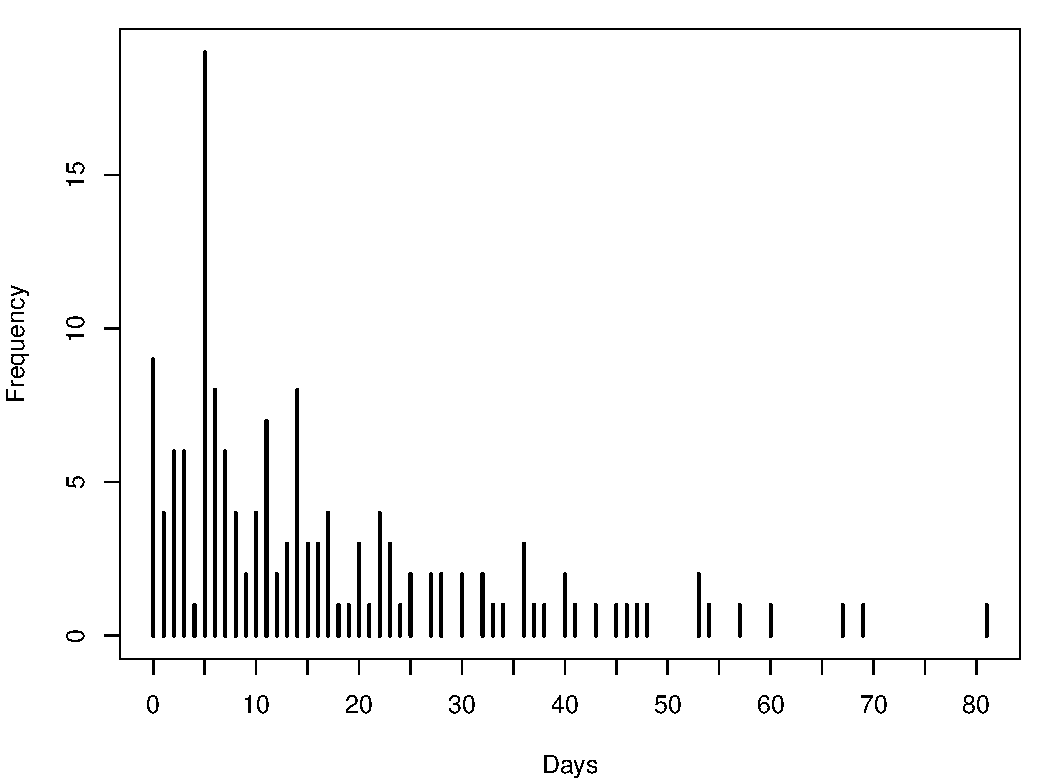
\includegraphics{delete-this-image}
%\caption{\label{fig:quine} Frequency distribution for number of days absent
%from school.}
%\end{figure}


%As a first model for the \code{quine} data, we fit the basic Poisson regression
%model. (Note that JSS prefers when the second line of code is indented by two
%spaces.)
%%
%\begin{CodeChunk}
%\begin{CodeInput}
%R> m_pois <- glm(Days ~ (Eth + Sex + Age + Lrn)^2, data = quine,
%+    family = poisson)
%\end{CodeInput}
%\end{CodeChunk}
%%
%Hence, the full summary of that model is shown below.
%%
%\begin{CodeChunk}
%\begin{CodeInput}
%R> summary(m_nbin)
%\end{CodeInput}
%\begin{CodeOutput}
%Call:
%glm.nb(formula = Days ~ (Eth + Sex + Age + Lrn)^2, data = quine, 
%    init.theta = 1.60364105, link = log)
%
%Coefficients: (1 not defined because of singularities)
%            Estimate Std. Error z value Pr(>|z|)    
%(Intercept)  3.00155    0.33709   8.904  < 2e-16 ***
% ...
%\end{CodeOutput}
%\end{CodeChunk}
%
%
%
%Here is another example of code:
%\begin{Code}
%glm(formula, data, subset, na.action, weights, offset,
%  family = gaussian, start = NULL, control = glm.control(...),
%  model = TRUE, y = TRUE, x = FALSE, ...)
%\end{Code}


%\begin{leftbar}
%As the synopsis above is a code listing that is not meant to be executed,
%one can use either the dedicated \verb|{Code}| environment or a simple
%\verb|{verbatim}| environment for this. Again, spaces before and after should be
%avoided.
%\end{leftbar}


%% -- Main Program ---------------------------------------------------------
% \section{Main Program} \label{sec:main}
% Renamed as Example session

\section{Example session} \label{sec:main}

A demonstration of analysis is shown in \verb|FCVAR_replication_JNP2014.R| and it serves as an example of what a typical session of model specification, estimation and testing can include. This code replicates ``Table 4: FCVAR results for Model 1'' from \cite{JNP2014} and follows the empirical procedure developed in that paper. This procedure includes the following steps:

\begin{enumerate}
\item Importing data
\item Choosing estimation options
\item Lag selection
\item Cointegration rank selection
\item Model estimation
\item Hypothesis testing
\end{enumerate}

% Understood by R users:
% i.e. don't open the package unless you want to know what's in it.
% 
%It is important to note that all necessary commands for file execution and option modification can be called from this script. All other files contained in the package (described in detail in the next section) do not require any modification by the user.

% Instructions not necessary: in package documentation
% 
%To accommodate the sequential nature of the procedure, the main file is broken up into \textit{code sections}\footnote{For more information see \url{ http://www.mathworks.com/help/MATLAB/MATLAB_prog/run-sections-of-programs.html}}. These \textit{code sections}, known as \textit{cells} in previous versions of MATLAB, allow the user to execute specific parts of a script individually. Each of the \textit{code sections} are delimited by a double comment \verb|%%| and the section header. 


\subsection{Importing data}

The first step is importing the data. Executing the code 
% in Listing~\ref{data}, 
shown below assigns data from the external dataset \verb|votingJNP2014|, which is available with the package. 

%\lstset{firstnumber=last}
%\begin{lstlisting}[frame=single,caption={Importing data}, label = data]
%\begin{CodeChunk} 
%\begin{CodeInput}
%\begin{Code}
%R> data <- read.csv('data_JNP2014.csv')
%R> x1 <- data(, c(1, 3, 5)) 
%R> x2 <- data(, [2 3 5]) 
%R> x3 <- data(, [1 2 3 5])
%R> x4 <- data(, [1 3 4 5 6])
%R> x5 <- data(, [2 3 4 5 6])
%R> x6 <- data(, [1 2 3 4 5 6])
%\end{Code}
%\end{CodeInput}
%\end{CodeChunk}
%\end{lstlisting}

%\begin{leftbar}
%Better to use names of variables for clarity. 
%Are we actually using these matrices? 
%Maybe we don't need numbers. 
%I think we only use \verb|x1|, so we should just call it \verb|x|.
%Finally, the actual command for a user will be from a data folder in the package. 
%\end{leftbar}

\begin{Code}
R> x1 <- votingJNP2014[, c("lib", "ir_can", "un_can")]
\end{Code}

% Old version, example for user's data:
% But this would not be included here.  
%\begin{Code}
%R> data <- read.csv('data_JNP2014.csv')
%R> x1 <- data[, c("lib", "ir_can", "un_can")]
%\end{Code}


The columns of the full dataset contain the following variables: (1) aggregate support for the Liberal party, (2) aggregate support for the Conservative party, (3) Canadian 3-month T-bill rates, (4) US 3-month T-bill rates, (5) Canadian unemployment rate, and (6) US unemployment rate. 
%Since each of the models in JNP (2014) contain different combinations of these variables, the relevant columns of \verb|data| for each model are assigned to different matrices of variables named \verb|x1| through \verb|x6|. 
This example uses the variables in the first, third and fifth columns. 

\subsection{Choosing options}
\label{subsec choosing options}

Once the data is imported, the user sets the program options. The script contains two sets of options: variables set for function arguments in the script itself and model/estimation related options. 
% Listing ~\ref{intl} shows the first of set of options. 
The first of set of options is as follows. 
% 
%\begin{lstlisting}[frame=single,caption={Initialization of local variables}, label = intl]
% NOTE: Alignment is achieved by counting the number of characters, including spaces.
% That is, this table looks ragged here but aligned in the document:
\begin{Code}
p               <- ncol(x1) 
kmax            <- 3
order           <- 12
printWNtest     <-  1
\end{Code}
%\end{lstlisting}

The variable \verb|kmax| determines the highest lag order for the sequential testing that is performed in the lag selection, whereas \verb|p| is the dimension of the system. 
% The other variables are self-explanatory.
The \verb|order| specifies the number of lags used for the white noise test in lag selection, 
while \verb|printWNtest| indicates whether to print results of white noise tests post-estimation. 

The next set of initialization commands
% , shown in Listing~\ref{intl2}, 
assign values to the variables contained in the object \verb|opt| defined by the function \fct{FCVARoptions}. 

%\begin{leftbar} 
%I wonder if we should leave some of this to the package documentation. 
%Maybe for this article, we should concentrate on the options that are necessary for the examples below. 
%Besides, JSS style prefers code blocks do not have comments, i.e. state it in the text. 
%We could say that ``the rest of the options are described in the package documentation''. 
% 
%Verdict: Here is a trimmed-down version. 
%I hope JSS is flexible about the comments, which I think are justified here.
%\end{leftbar}

%\begin{lstlisting}[frame=single,caption={Choosing estimation options}, label = intl2]
\begin{Code}
# Define variable to store estimation options.
opt              <- EstOptions() 
opt$dbMin        <- c(0.01, 0.01) # lower bound for d, b.
opt$dbMax        <- c(2.00, 2.00) # upper bound for d, b.
opt$unrConstant  <- 0   # include an unrestricted constant? 
opt$rConstant    <- 0   # include a restricted constant? 
opt$levelParam   <- 1   # include level parameter? 
opt$constrained  <- 0   # impose restriction dbMax >= d >= b >= dbMin? 
opt$restrictDB   <- 1   # impose restriction d = b ? 
opt$db0          <- c(0.80, 0.80) # set starting values for optimization.
opt$N            <- 0   # number of initial values to condition upon.
opt$print2screen <- 1   # print output.
opt$printRoots   <- 1   # do not print roots of characteristic polynomial.
opt$plotRoots    <- 1   # do not plot roots of characteristic polynomial.
opt$gridSearch   <- 1   # For more accurate estimation, perform a grid search.
                        # This will make estimation take longer.
opt$plotLike     <- 0   # Plot the likelihood (if gridSearch <- 1).
opt$progress     <- 0   # Show grid search progress indicator waitbar.
opt$updateTime   <- 0.5 # How often progress is updated (seconds).

# Store the options to reset them in between hypothesis tests.
DefaultOpt <- opt 
\end{Code}
%\end{lstlisting}

The first line initializes the object \verb|opt| and assigns all of the default options set in \verb|FCVARoptions|. The user can see the full set of options by typing \verb|DefaultOpt| (or \verb|opt| after initialization) in the command line. % Listing~\ref{intl2} 
The code block above 
shows how to easily change any of the default options. Defining the program options in this way allows the user to create and store several option objects with different attributes. This can be very convenient when, for example, performing the same hypothesis tests on different data sets. 

The set of available options can be broken into several categories: numerical optimization, model deterministics and restrictions, output and grid search.
% , and $p$~values for the rank test. 
% These are obtained internally from the \pkg{fracdist} package, with no user input. 
We recommend that only advanced users make changes to the numerical optimization options. Adding deterministics requires setting the variable corresponding to the type of deterministic component to 1. For instance, in the present example, a model estimated with options \verb|opt| will include the level parameter $\mu$ but no restricted or unrestricted constant. Output variables refer to either printing or plotting various information post-estimation and usually take values $1$ or $0$ (on or off). For example, if the user is not interested in the estimates of $\Gamma$, they can be suppressed by setting \verb|opt$printGammas <- 0|.

The bounds on the parameter space for $d$ and $b$ are specified in \verb|opt$dbMin| and \verb|opt$dbMax|. In this example, these are both specified as 2-dimensional column vectors, in which case the first element specifies the bound on $d$ and the second element the bound on $b$. Alternatively, one can set \verb|opt$dbMin| and \verb|opt$dbMax| as scalars, which imposes the same bounds on $d$ and $b$. 

An important feature in this package is the ability to pre-estimate by using a grid search. If the user selects this option, they can view progress by setting \verb|opt$progress| to $1$ (waitbar) or $2$ (output in command line). The minimum frequency of these updates is set by \verb|opt$updateTime|. The user also has the option (\verb|opt$plotLike|) to view a plot of the likelihood over $d$ and/or $b$ after the grid search completes. The output of the grid search is a preliminary estimate of the fractional parameters. These are used as starting values in the subsequent numerical optimization, and the bounds on $d$ and $b$ are set to these starting values plus/minus $0.1$ but still within the original \verb|dbMin| and \verb|dbMax| settings.

\begin{leftbar}
Warning: The current package does not have the following functionality. 
It could be implemented but I imagine there already exists something in R that can serve this role. 
However, I think I don't quite understand the problem without it. 
Can you provide an example? 
\end{leftbar}

As of v.1.4.0, the new option \verb|opt$LocalMax| allows more control over the grid search. If \verb|opt$LocalMax <- 0|, the function \fct{FCVARlikeGrid} returns the parameter values corresponding to the global maximum of the likelihood on the grid. If \verb|opt$LocalMax <- 1|, then \fct{FCVARlikeGrid} returns the parameter values for the local maximum corresponding to the highest value of $b$. This is meant to alleviate the identification problem discussed in \citet[Section 2.3]{johniel2010} and \cite{Carlini2014}. As of v.1.4.0, the default setting is \verb|opt$LocalMax <- 1|.

Another option is the addition of a line search to the switching algorithm for estimation of models with restrictions on $\alpha$ and/or $\beta$. This is added via the option \verb|opt$LineSearch <- 1| and is the default. See \citet[Section 2.2]{Doornik2016} for details.

%\begin{leftbar}
%Removing this to reflect our updated strategy for the $p$~values for cointegration rank tests
%-- it simply calls the \pkg{fracdist} package and calculates the $p$~values. 
%This is much better than calling the \pkg{Rcpp} package because it avoids the inevitable probelms with platform, compiler and software dependencies. 
%Besides, CRAN doesn't like packages to make system calls because it makes assumptions about the user's setup and leads to the above problems with dependencies. 
%\end{leftbar}
%
%In order to automatically obtain $p$~values for cointegration rank tests when $b>0.5$, the user needs to download and install the necessary program 
%% (see Section~\ref{sec obtaining}). 
%(see Section~\ref{sec:fdpval}). 
%The last option, \verb|opt$progLoc|, identifies the location of that program.

After all options have been set, the last line 
% in Listing~\ref{intl2} 
stores them in \verb|DefaultOpt| so that the user can recall them at any point in the estimation. This is particularly useful if the user wants to change only a few options in between estimations.


\subsection{Lag-order selection}

Once the options are set, the user moves to the next step, which involves choosing the appropriate lag order. The relevant information is obtained with a call to \fct{FCVARlagSelect}
%, shown in Listing~\ref{FCVARlagSelect}, 
which performs estimation of models with lag-orders from $0$ to \verb|kmax|. The program performs lag selection on the full-rank unrestricted model. 

% The output generated by this function is shown below. 
\begin{leftbar}
Our \proglang{MATLAB} output is wider than 80 characters. This will sometimes be a problem. 
In particular, in the JSS draft, 80 characters in the \verb|CodeChunk| environment will fit well within the margins.
What follows is the revised format of the output.
\end{leftbar}

%\begin{lstlisting}[frame=single,caption={Lag selection}, label = FCVARlagSelect]
%\end{lstlisting}
\begin{CodeChunk} 
\begin{CodeInput}
R> FCVARlagSelectStats <- FCVARlagSelect(x1, kmax, p, order, opt)
\end{CodeInput}
\begin{CodeOutput}
--------------------------------------------------------------------------------
                        Lag Selection Results 
--------------------------------------------------------------------------------
Dimension of system:       3     Number of observations in sample:          316 
Order for WN tests:       12     Number of observations for estimation:     316 
Restricted constant:      No     Initial values:                              0
Unrestricted constant:    No     Level parameter:                           Yes
--------------------------------------------------------------------------------
Parameter Estimates and Information Criteria:
--------------------------------------------------------------------------------
 k  r    d    b      LogL     LR    pv    AIC       BIC
 3  3 0.676 0.676  456.42   7.31 0.605  -832.85   -682.62 
 2  3 0.581 0.581  452.77  20.59 0.015  -843.53*  -727.11 
 1  3 1.043 1.043  442.47  56.99 0.000  -840.94   -758.31*
 0  3 1.036 1.036  413.97   0.00 0.000  -801.95   -753.12 
--------------------------------------------------------------------------------
Tests for Serial Correlation of Residuals: 
--------------------------------------------------------------------------------
 k   pmvQ  pQ1   pLM1  pQ2   pLM2  pQ3   pLM3
 3   0.94  0.72  0.46  0.49  0.89  0.51  0.47
 2   0.82  0.69  0.45  0.29  0.75  0.54  0.40
 1   0.34  0.75  0.52  0.15  0.58  0.34  0.18
 0   0.00  0.01  0.01  0.00  0.08  0.37  0.17
--------------------------------------------------------------------------------
\end{CodeOutput}
\end{CodeChunk} 

Estimates of $d$ and $b$ are reported for each lag ($k$) with rank ($r$) set to the number of variables in the system. Note that in this example the restriction $d=b$ has been imposed. The log-likelihood for each lag is shown in column \verb|LogL|. The likelihood ratio test-statistic \verb|LR| is for the null hypothesis $\Gamma_k = 0$ with $p$~value reported in column \verb|pv|. This is followed by AIC and BIC information criteria. The columns in the next block provide $p$~values for white noise tests on the residuals. The first $p$~value, \verb|pmvQ|, is for the multivariate Q-test followed by univarite Q-tests as well as LM tests on the $p$ individual residuals; that is, \verb|pQ1| and \verb|pLM1| are the $p$~values for the residuals in the first equation, \verb|pQ2| and \verb|pLM2| are for the residuals in the second equation, and so on. 


\subsection{Cointegration rank testing}

The user now chooses the lag-order based on the information provided above and can move to the next step, which is cointegration rank testing. 
% The next code section is shown in listing~\ref{RankSelect}. T
In the next code block, the user first assigns the lag augmentation, $k = 2$ in this case, and then calls the function \fct{FCVARrankTests}. 

%% --------- COINTEGRATION RANK TESTING ---------- %
%Executing the code in Listing~\ref{RankSelect} produces the following output. 

%\begin{lstlisting}[frame=single,caption={Cointegration rank testing}, label = RankSelect]
\begin{CodeChunk} 
\begin{CodeInput}
R> k <- 2
R> rankTestStats <- FCVARrankTests(x1, k, opt)
\end{CodeInput}
\begin{CodeOutput}
--------------------------------------------------------------------------------
             Likelihood Ratio Tests for Cointegrating Rank                               
--------------------------------------------------------------------------------
Dimension of system:       3     Number of observations in sample:          316 
Number of lags:            2     Number of observations for estimation:     316 
Restricted constant:      No     Initial values:                              0
Unestricted constant:     No     Level parameter:                           Yes
--------------------------------------------------------------------------------
Rank     d      b     Log-likelihood   LR statistic   P-value
 0     0.643  0.643          440.040         25.454     0.043
 1     0.569  0.569          451.174          3.186     0.820
 2     0.576  0.576          452.707          0.120     0.947
 3     0.581  0.581          452.767           ----      ----
--------------------------------------------------------------------------------
\end{CodeOutput}
\end{CodeChunk} 


The first block of output provides a summary of the model specification. The second block provides the test results relevant for selecting the appropriate rank. 
These include likelihood ratio tests for a restriction to a cointegrating rank against an unrestricted model with full rank. 
% 
The $p$~values are calculated by the \pkg{fracdist} package, which obtains simulated $p$~values from \cite{mackinnon2014numerical}. 
% 
The table is meant to be read sequentially from lowest to highest rank, i.e.\ from top to bottom. Since we can reject the null of rank 0 against the alternative of rank 3 we move to the test of rank 1 against rank 3. This test fails to reject with a $p$~value of $0.820$, so this is the appropriate choice in this case.


\subsection{Unrestricted model estimation}

With the rank and lag selected, the user can now move to the next code section. 
% , shown in Listing~\ref{unrEst}.
% 

% Split this up below:
%% --------- UNRESTRICTED MODEL ESTIMATION ---------- %
%\begin{lstlisting}[frame=single,caption={Unrestricted model estimation}, label = unrEst]
%\begin{CodeChunk} 
%\begin{CodeInput}
%R> r <- 1
%R> opt1 <- DefaultOpt
%R> m1 <- FCVARestn(x1, k, r, opt1)
%R> MVWNtest(m1$Residuals, order, printWNtest)
%\end{CodeInput}
%\end{CodeChunk} 
%\end{lstlisting}
% 
Here the user first specifies the choice for the rank based on the previously performed cointegrating rank tests (thus setting $r=1$ in this example). Next, the default options set in the initialization, see Section \ref{subsec choosing options}, are assigned to \verb|opt1|, which is used as an argument in the call to the function \fct{FCVARestn}. This function is the main part of the program since it performs the estimation of the parameters, obtains model residuals and standard errors, and calculates many other relevant components such as the number of free parameters and the roots of the characteristic polynomial. If \verb|opt1$print2screen <- 1| then, in addition to storing all of these results in the list \verb|m1|, the function outputs the estimation results to the command window. To see a list of variables stored in \verb|m1|, the user can type \verb|m1| in the command line. 

The program output is shown below. It begins with a table summarizing relevant model specifications and then the coefficients and their standard errors. The roots of the characteristic polynomial are displayed at the bottom. 

\begin{leftbar}
I trimmed the output to 80 characters wide. 
There were no numbers in that range, only comments. 
Besides, it is no coincidence that only the output in the first 80 characters lies in the margins of a JSS article.
The output from the software should lie within this range. 
\end{leftbar}

\begin{CodeChunk} 
\begin{CodeInput}
R> r <- 1
R> opt1 <- DefaultOpt
R> m1 <- FCVARestn(x1, k, r, opt1)
\end{CodeInput}
\begin{CodeOutput}
--------------------------------------------------------------------------------
                      Fractionally Cointegrated VAR: Estimation Results                              
--------------------------------------------------------------------------------
Dimension of system:       3      Number of observations in sample:          316 
Number of lags:            2      Number of observations for estimation:     316 
Restricted constant:      No      Initial values:                              0
Unrestricted constant:    No      Level parameter:                           Yes
Starting value for d:    0.800    Parameter space for d: (0.010 , 2.000) 
Starting value for b:    0.800    Parameter space for b: (0.010 , 2.000) 
--------------------------------------------------------------------------------
Cointegrating rank:            1  AIC:              -848.348 
Log-likelihood:          451.174  BIC:              -746.943 
log(det(Omega_hat)):     -11.369  Free parameters:        27 
--------------------------------------------------------------------------------
    Fractional parameters:                                                                             
--------------------------------------------------------------------------------
    Coefficient               Estimate                Standard error 
--------------------------------------------------------------------------------
         d                       0.569                      0.049                
--------------------------------------------------------------------------------
--------------------------------------------------------------------------------
    Cointegrating equations (beta):                                                                  
--------------------------------------------------------------------------------
      Variable        CI equation 1  
--------------------------------------------------------------------------------
        Var1              1.000     
        Var2              0.111     
        Var3             -0.240     
--------------------------------------------------------------------------------
Note: Identifying restriction imposed.                                                               
--------------------------------------------------------------------------------
    Adjustment matrix (alpha):                                                                         
--------------------------------------------------------------------------------
      Variable        CI equation 1  
--------------------------------------------------------------------------------
        Var 1            -0.180     
         SE 1         (   0.064  )  
        Var 2             0.167     
         SE 2         (   0.194  )  
        Var 3             0.037     
         SE 3         (   0.014  )  
--------------------------------------------------------------------------------
Note: Standard errors in parenthesis.                                                                
--------------------------------------------------------------------------------
    Long-run matrix (Pi):                                                                       
--------------------------------------------------------------------------------
      Variable         Var 1          Var 2          Var 3   
--------------------------------------------------------------------------------
      Var 1           -0.180         -0.020          0.043    
      Var 2            0.167          0.019         -0.040    
      Var 3            0.037          0.004         -0.009    
--------------------------------------------------------------------------------

--------------------------------------------------------------------------------
    Level parameter (mu):                                                                         
--------------------------------------------------------------------------------
        Var 1            -0.345     
         SE 1         (   0.069  )  
        Var 2            11.481     
         SE 2         (   0.548  )  
        Var 3            -2.873     
         SE 3         (   0.033  )  
--------------------------------------------------------------------------------
Note: Standard errors in parenthesis (from numerical Hessian) 
      but asymptotic distribution is unknown. 
--------------------------------------------------------------------------------
    Lag matrix 1 (Gamma_1):                                                                            
--------------------------------------------------------------------------------
      Variable         Var 1          Var 2          Var 3   
--------------------------------------------------------------------------------
      Var 1            0.276         -0.032         -0.510    
       SE 1        (   0.160  )   (   0.026  )   (   0.513  )  
      Var 2           -0.148          1.126         -3.289    
       SE 2        (   0.378  )   (   0.196  )   (   1.975  )  
      Var 3           -0.052          0.008          0.711    
       SE 3        (   0.022  )   (   0.005  )   (   0.170  )  
--------------------------------------------------------------------------------
Note: Standard errors in parentheses.                                                                
--------------------------------------------------------------------------------
    Lag matrix 2 (Gamma_2):                                                                            
--------------------------------------------------------------------------------
      Variable         Var 1          Var 2          Var 3   
--------------------------------------------------------------------------------
      Var 1            0.566          0.106          0.608    
       SE 1        (   0.182  )   (   0.045  )   (   0.612  )  
      Var 2            0.493         -0.462          0.457    
       SE 2        (   0.562  )   (   0.198  )   (   2.628  )  
      Var 3           -0.039         -0.020          0.318    
       SE 3        (   0.033  )   (   0.008  )   (   0.143  )  
--------------------------------------------------------------------------------
Note: Standard errors in parentheses.                                                                
--------------------------------------------------------------------------------
--------------------------------------------------------------------------------
    Roots of the characteristic polynomial                                                           
--------------------------------------------------------------------------------
    Number     Real part    Imaginary part       Modulus                                             
--------------------------------------------------------------------------------
       1         -2.893         -0.000            2.893                                        
       2         -1.522         -0.000            1.522                                        
       3          1.010         -0.927            1.371                                        
       4          1.010          0.927            1.371                                        
       5          1.107          0.000            1.107                                        
       6          1.000          0.000            1.000                                        
       7          1.000          0.000            1.000                                        
       8          0.944         -0.261            0.980                                        
       9          0.944          0.261            0.980                                        
--------------------------------------------------------------------------------

--------------------------------------------------------------------------------
Restrictions imposed on the following parameters:
- Psi. For details see "options$R_psi"
--------------------------------------------------------------------------------
\end{CodeOutput}
\end{CodeChunk} 

At the end of the output, a notice is printed to remind the user that restrictions were imposed on \verb|Psi|, i.e.\ on $(d,b)$. In this case, this is the restriction $d=b$ imposed via \verb|opt$restrictDB <- 1|.

In addition to the coefficient estimates, we are also interested in testing the model residuals for serial correlation.
%
After the unrestricted model has been estimated, this code section concludes with a call to \fct{MVWNtest}, which performs a series of white noise tests on the residuals and prints the output in the command window.
%
The results of the white noise tests
%, called in the last line of Listing \ref{unrEst}, 
are shown below. For each residual both the Q- and LM-test statistics and their $p$~values are reported, in addition to the multivariate Q-test and $p$~value in the first line of the table. From the output of this table we can conclude that there does not appear to be any problems with serial correlation in the residuals.


\begin{CodeChunk} 
\begin{CodeInput}
R> MVWNtest_m1 <- MVWNtest(m1$Residuals, order, printWNtest)
\end{CodeInput}
\begin{CodeOutput}
       White Noise Test Results (lag = 12)
---------------------------------------------
Variable |       Q  P-val |      LM  P-val  |
---------------------------------------------
Multivar |  97.879  0.747 |     ----  ----  |
Var1     |   9.300  0.677 |  11.238  0.509  |
Var2     |  14.450  0.273 |   8.568  0.739  |
Var3     |  10.591  0.564 |  12.265  0.425  |
---------------------------------------------
\end{CodeOutput}
\end{CodeChunk} 

Because \verb|opt$plotRoots <- 1| in the options, 
% in Listing~\ref{intl2}, 
the roots of the characteristic polynomial is also plotted along with the unit circle and the transformed unit circle, $\mathbb{C}_{\hat{b}}$, see \cite{Johansen2008}. 
The plot is shown in Figure~\ref{fig:Roots}.
% Note that the axes of the plot are fixed, and therefore very large roots may not be shown in the plot (in this example, the real root \verb|-2.893|). This should not be a problem since such roots will always be well outside the transformed unit circle.


\begin{figure}[H]
  \centering
  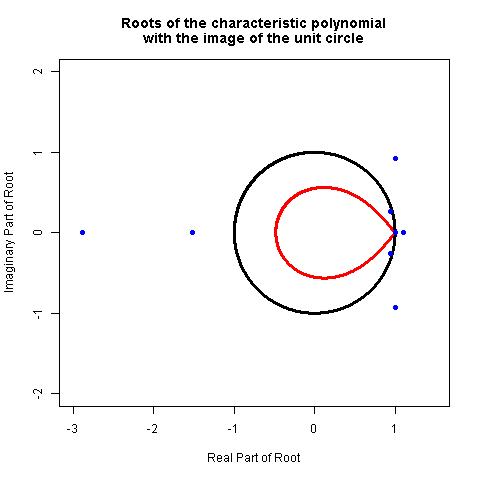
\includegraphics[scale = .6, keepaspectratio=true]{Figures/roots.png}
  \caption{Roots of characteristic polynomial}
  \label{fig:Roots}
\end{figure}

Furthermore, the estimation was performed with the grid search and the plot option selected, i.e.\ with \verb|opt$gridSearch <- 1| and \verb|opt$plotLike <- 1|, which produces a plot of the log-likelihood. The plot for this model is shown in Figure~\ref{fig:m1_likelihood}.

\begin{figure}[H]
  \centering
  
\includegraphics[scale = .6, keepaspectratio=true]{Figures/m1_likelihood.png}
  \caption{Plot of log-likelihood}
  \label{fig:m1_likelihood}
\end{figure}

The complete results for the unrestricted model are stored in the list \verb|m1| and can be accessed anytime. For instance, if the user would like to perform a more careful analysis of the residuals they are stored in \verb|m1$Residuals|.

\subsection{Hypothesis testing}
\label{subsec hypo}

We now move into the hypothesis testing section of the code where we can test several restricted models and perform inference. For restricted model estimation the grid search option is switched off because computation can be very slow, especially in the presence of the level parameter. However, if the user wishes to verify the accuracy of the results or if estimates are close to the upper or lower bound, the grid search option can resolve these issues and give the user additional insight about the behaviour of the likelihood.

All hypotheses are defined as shown in \eqref{R psi}--\eqref{R beta}. The first hypothesis test is $\mathscr{H}_d^1$ (for precise definitions of each hypothesis, please see \cite{JNP2014}), 
%and it is shown in Listing~\ref{Hdb1}. 
shown below. 

%% --------- IMPOSE RESTRICTIONS AND TEST THEM ---------- %
%\begin{lstlisting}[frame=single,caption={Hypothesis $\mathscr{H}_d^1$}, label = Hdb1]
\begin{Code}
R> opt1 <- DefaultOpt
R> opt1$R_psi <- matrix(c(1, 0), nrow = 1, ncol = 2)
R> opt1$r_psi <- 1
R> m1r1 <- FCVARestn(x1, k, r, opt1)
R> MVWNtest_m1r1 <- MVWNtest(m1r1$Residuals, order, printWNtest)
R> Hdb <- FCVARhypoTest(m1, m1r1)
\end{Code}
%\end{lstlisting}

Here we test the CVAR model (null hypothesis $d=b=1$) against the FCVAR model (alternative hypothesis $d=b\ne 1$). Since \verb|opt1$restrictDB <- 1| was selected in the choice of options,
% in Listing \ref{intl2}, 
the restriction that $d=b$ is already imposed. Thus, the user needs to only impose an additional restriction that either $d$ or $b$ is equal to one. In this example, the restriction that $d=1$ is imposed by setting \verb|opt1$R_psi = [1 0]| and \verb|opt1$r_psi = 1|, but the result would be the same if $b=1$ were imposed instead. The restricted model is then estimated and the results are stored in the MATLAB structure \verb|m1r1|. As before, the user can perform a series of white noise tests on the residuals by calling the \fct{MVWNtest} function. The next step is to perform the actual test. With the results structures from the restricted and unrestricted models, the user can call the function \fct{FCVARhypoTest} and perform an LR test. This function takes the two model result structures as inputs, automatically compares the number of free parameters to obtain the degrees of freedom, computes the LR test statistic, and displays the output. The results of this test are then stored in the list \verb|Hdb| and can be accessed at any time.

Since the output of the estimated model and the white noise tests are similar to the previous example, we only show the output from the hypothesis test. 

\begin{verbatim}
Likelihood ratio test results:
Unrestricted log-likelihood: 451.174
Restricted log-likelihood:   442.027
Test results (df = 1):
LR statistic: 	 18.295
P-value: 	 0.000
\end{verbatim}

The log-likelihoods from both models are reported, along with the degrees of freedom, the LR test statistic, and its $p$~value. In this case the test clearly rejects the null hypothesis that the model is a CVAR. For more significant digits, or to access any of these values from the command window, the user can type \verb|Hdb|.

The next hypothesis of interest is $\mathscr{H}_{\beta}^1$, which is a zero restriction on the first element of the cointegration vector.

%\begin{lstlisting}[frame=single,caption={Hypothesis $\mathscr{H}_{\beta}^1$}, label = Hb1]
\begin{Code}
R> opt1 <- DefaultOpt
R> opt1$R_Beta <- matrix(c(1, 0, 0), nrow = 1, ncol = 3)
R> m1r2 <- FCVARestn(x1, k, r, opt1)
R> MVWNtest_m1r2 <- MVWNtest(m1r2$Residuals, order, printWNtest)
R> Hbeta1 <- FCVARhypoTest(m1, m1r2)
\end{Code}
%\end{lstlisting}

Since the object \verb|opt1| has the restriction $d=b=1$ stored, the first step is to reset the options to default. The restriction on $\beta$ is then specified as in \eqref{R beta}. There are two things to note here. First, the column length of $R_{\beta}$ must equal $p_1 r$, where $p_1=p+1$ if a restricted constant is present and $p_1=p$ otherwise; recall that $p$ is the number of variables in the system and $r$ is the number of cointegrating vectors. Second, zero restrictions are the default and automatically imposed when $r_{\beta}$ is empty. Therefore, the user only needs to specify $r_{\beta}$ if it includes non-zero elements. Recall that for restrictions on $\alpha$ only $r_\alpha = 0$ is allowed so that there is no need to specify $r_\alpha$. As before, the restricted model is estimated with results stored in \verb|m1r2|, the residuals are tested for white noise, and the model under the null is tested against the unrestricted model \verb|m1| with results stored in \verb|Hbeta1|.

Again, since the estimation output is similar to the first example, we only show the results of the hypothesis test here. With a $p$~value close to zero, this hypothesis is also strongly rejected.

\begin{verbatim}
Likelihood ratio test results:
Unrestricted log-likelihood: 451.174
Restricted log-likelihood:   444.395
Test results (df = 1):
LR statistic: 	 13.557
P-value: 	 0.000
\end{verbatim}

Next, we move to tests on $\alpha$. 
In this case, we test restriction that political variable is long-run exogenous.

%\begin{lstlisting}[frame=single,caption={Hypothesis $\mathscr{H}_{\alpha}^1$}, label = Ha1]
\begin{Code}
R> opt1 <- DefaultOpt
R> opt1$R_Alpha <- matrix(c(1, 0, 0), nrow = 1, ncol = 3)
R> opt1$gridSearch <- 0
R> m1r3 <- FCVARestn(x1, k, r, opt1)
R> MVWNtest_m1r3 <- MVWNtest(m1r3$Residuals, order, printWNtest)
R> Halpha1 <- FCVARhypoTest(m1, m1r3)
\end{Code}
%\end{lstlisting}

Again we first reset \verb|opt1| to the default options to clear previously imposed restrictions. Note that, if it were the case that we failed to reject $\mathscr{H}_{\beta}^1$ and wanted to leave it imposed while adding a restriction on $\alpha$, we could either omit the first line \verb|opt1 <- DefaultOpt|, or we could replace it with \verb|opt1 <- m1r2$options|. The latter assignment is preferred in this case because it is explicit about which model options we are leaving imposed.

The hypothesis $\mathscr{H}_{\alpha}^1$ is tested in the exact same way as before, only now we are changing the variable $R_{\alpha}$ instead of $R_{\beta}$. The results are shown below and we can see that this hypothesis is also rejected.

\begin{verbatim}
Likelihood ratio test results:
Unrestricted log-likelihood: 451.174
Restricted log-likelihood:   446.086
Test results (df = 1):
LR statistic: 	 10.176
P-value: 	 0.001
\end{verbatim}

We next move to the remaining long-run exogeneity tests, $\mathscr{H}_{\alpha}^2$ and $\mathscr{H}_{\alpha}^3$, shown
% in Listings \ref{Ha2} and \ref{Ha3}, respectively. 
the examples below.
% The results of the tests are shown below each listing.
The hypothesis $\mathscr{H}_{\alpha}^2$ tests that the interest-rate is long-run exogenous.

%\begin{lstlisting}[frame=single,caption={Hypothesis $\mathscr{H}_{\alpha}^2$}, label = Ha2]
%% Test restriction that interest-rate is long-run exogenous.
\begin{CodeChunk} 
\begin{CodeInput}
R> opt1 <- DefaultOpt
R> opt1$R_Alpha <- matrix(c(0, 1, 0), nrow = 1, ncol = 3)
R> opt1$gridSearch <- 0
R> m1r4 <- FCVARestn(x1, k, r, opt1)
R> MVWNtest_m1r4 <- MVWNtest(m1r4$Residuals, order, printWNtest)
R> Halpha2 <- FCVARhypoTest(m1, m1r4)
\end{CodeInput}
\begin{CodeOutput}
Likelihood ratio test results:
Unrestricted log-likelihood: 451.174
Restricted log-likelihood:   450.857
Test results (df = 1):
LR statistic: 	 0.633
P-value: 	 0.426
\end{CodeOutput}
\end{CodeChunk}  


Next, we test the hypothesis $\mathscr{H}_{\alpha}^3$ that unemployment is long-run exogenous.

%\begin{lstlisting}[frame=single,caption={Hypothesis $\mathscr{H}_{\alpha}^3$}, label = Ha3]
\begin{CodeChunk} 
\begin{CodeInput}
R> opt1 <- DefaultOpt
R> opt1$gridSearch <- 0
R> opt1$R_Alpha <- matrix(c(0, 0, 1), nrow = 1, ncol = 3)
R> m1r5 <- FCVARestn(x1, k, r, opt1)
R> MVWNtest_m1r5 <- MVWNtest(m1r5$Residuals, order, printWNtest)
R> Halpha3 <- FCVARhypoTest(m1, m1r5)
\end{CodeInput}
\begin{CodeOutput}
Likelihood ratio test results:
Unrestricted log-likelihood: 451.174
Restricted log-likelihood:   446.184
Test results (df = 1):
LR statistic: 	 9.979
P-value: 	 0.002
\end{CodeOutput}
\end{CodeChunk}  

The only hypothesis that we fail to reject is $\mathscr{H}_{\alpha}^2$, under which interest rates are long-run exogenous. 
After having estimated all of the restricted models of interest, we provide the full estimation output for the model \verb|m1r4|, with the restriction imposed for $\mathscr{H}_{\alpha}^2$. 
Note from the output that $\alpha_2 = 0$ as imposed by the restriction.

\begin{verbatim}
--------------------------------------------------------------------------------
                      Fractionally Cointegrated VAR: Estimation Results                              
--------------------------------------------------------------------------------
Dimension of system:       3      Number of observations in sample:          316 
Number of lags:            2      Number of observations for estimation:     316 
Restricted constant:      No      Initial values:                              0
Unrestricted constant:    No      Level parameter:                           Yes
Starting value for d:    0.800    Parameter space for d: (0.010 , 2.000) 
Starting value for b:    0.800    Parameter space for b: (0.010 , 2.000) 
--------------------------------------------------------------------------------
Cointegrating rank:            1  AIC:              -849.715 
Log-likelihood:          450.857  BIC:              -752.065 
log(det(Omega_hat)):     -11.367  Free parameters:        26 
--------------------------------------------------------------------------------
    Fractional parameters:                                                                             
--------------------------------------------------------------------------------
    Coefficient               Estimate                Standard error 
--------------------------------------------------------------------------------
         d                       0.575                      0.048                
--------------------------------------------------------------------------------
--------------------------------------------------------------------------------
    Cointegrating equations (beta):                                                                  
--------------------------------------------------------------------------------
      Variable        CI equation 1  
--------------------------------------------------------------------------------
        Var1              0.994     
        Var2              0.105     
        Var3             -0.181     
--------------------------------------------------------------------------------
    Adjustment matrix (alpha):                                                                         
--------------------------------------------------------------------------------
      Variable        CI equation 1  
--------------------------------------------------------------------------------
        Var 1            -0.189     
         SE 1         (   0.065  )  
        Var 2             0.000     
         SE 2         (   0.000  )  
        Var 3             0.039     
         SE 3         (   0.014  )  
--------------------------------------------------------------------------------
Note: Standard errors in parenthesis.                                                                
--------------------------------------------------------------------------------
    Long-run matrix (Pi):                                                                       
--------------------------------------------------------------------------------
      Variable         Var 1          Var 2          Var 3   
--------------------------------------------------------------------------------
      Var 1           -0.188         -0.020          0.034    
      Var 2            0.000          0.000          0.000    
      Var 3            0.039          0.004         -0.007    
--------------------------------------------------------------------------------

--------------------------------------------------------------------------------
    Level parameter (mu):                                                                         
--------------------------------------------------------------------------------
        Var 1            -0.310     
         SE 1         (   0.067  )  
        Var 2            11.538     
         SE 2         (   0.553  )  
        Var 3            -2.874     
         SE 3         (   0.033  )  
--------------------------------------------------------------------------------
Note: Standard errors in parenthesis (from numerical Hessian) 
      but asymptotic distribution is unknown. 
--------------------------------------------------------------------------------
    Lag matrix 1 (Gamma_1):                                                                            
--------------------------------------------------------------------------------
      Variable         Var 1          Var 2          Var 3   
--------------------------------------------------------------------------------
      Var 1            0.269         -0.032         -0.511    
       SE 1        (   0.157  )   (   0.026  )   (   0.507  )  
      Var 2           -0.013          1.115         -3.004    
       SE 2        (   0.345  )   (   0.189  )   (   1.909  )  
      Var 3           -0.053          0.008          0.694    
       SE 3        (   0.022  )   (   0.005  )   (   0.164  )  
--------------------------------------------------------------------------------
Note: Standard errors in parentheses.                                                                
--------------------------------------------------------------------------------
    Lag matrix 2 (Gamma_2):                                                                            
--------------------------------------------------------------------------------
      Variable         Var 1          Var 2          Var 3   
--------------------------------------------------------------------------------
      Var 1            0.570          0.104          0.585    
       SE 1        (   0.184  )   (   0.044  )   (   0.606  )  
      Var 2            0.685         -0.371          0.229    
       SE 2        (   0.508  )   (   0.159  )   (   2.509  )  
      Var 3           -0.043         -0.020          0.330    
       SE 3        (   0.032  )   (   0.008  )   (   0.138  )  
--------------------------------------------------------------------------------
Note: Standard errors in parentheses.                                                                
--------------------------------------------------------------------------------
--------------------------------------------------------------------------------
    Roots of the characteristic polynomial                                                           
--------------------------------------------------------------------------------
    Number     Real part    Imaginary part       Modulus                                             
--------------------------------------------------------------------------------
       1         -2.710         -0.000            2.710                                        
       2         -1.498         -0.000            1.498                                        
       3          1.130         -0.939            1.469                                        
       4          1.130          0.939            1.469                                        
       5          1.098          0.000            1.098                                        
       6          1.000          0.000            1.000                                        
       7          1.000          0.000            1.000                                        
       8          0.934         -0.281            0.976                                        
       9          0.934          0.281            0.976                                        
--------------------------------------------------------------------------------

--------------------------------------------------------------------------------
Restrictions imposed on the following parameters:
- Psi. For details see "options$R_psi"
- Alpha. For details see "options$R_Alpha"
--------------------------------------------------------------------------------


       White Noise Test Results (lag = 12)
---------------------------------------------
Variable |       Q  P-val |      LM  P-val  |
---------------------------------------------
Multivar |  97.674  0.752 |     ----  ----  |
Var1     |   9.083  0.696 |  11.268  0.506  |
Var2     |  14.937  0.245 |   9.339  0.674  |
Var3     |  10.725  0.553 |  12.237  0.427  |
---------------------------------------------
\end{verbatim}

Sometimes it is the case that the model output is not normalized with respect to the user's variable of interest, for example when restrictions are imposed on $\alpha$ or $\beta$. For this reason, we also include a code section that normalizes the output, i.e.\ imposes an identity matrix in the first $r \times r$ block of $\beta$. 
That is, $\hat{\alpha}$ is post multiplied by $G^{-1}$ so that $\pi= \hat{\alpha}(G^{-1})G\hat{\beta}' = ab'$\footnote{Let's revise this sentence to account for the changing definition of $\hat{\alpha}$ and $\hat{\beta}$ throughout the calculation}.
Of course, this code section should only be executed if it does not interfere with any restrictions imposed on the model.


%\begin{lstlisting}[frame=single,caption={Normalizing output}, label = normOut]
\begin{CodeChunk} 
\begin{CodeInput}
R> modelRstrct <- m1r4
R> G <- solve(modelRstrct$coeffs$betaHat[1:r, 1:r])
R> betaHatR <- modelRstrct$coeffs$betaHat %*% G
R> alphaHatR <- modelRstrct$coeffs$alphaHat %*% t(solve(G))
R> print("betaHatR' = ")
R> print(t(betaHatR), print.gap = 5)
R> print("alphaHatR' = ")
R> print(t(alphaHatR), print.gap = 5)
\end{CodeInput}
\end{CodeChunk}  


As an example of when this feature can be useful, consider model $\mathscr{H}_{\alpha}^2$. In the output above, we notice that the cointegrating vector has not been normalized (because restrictions are imposed). The user assigns the model of interest to the variable \verb|modelRstrct|, in this case \verb|m1r4|, and executes the commands. The output is shown below.

\begin{CodeChunk} 
\begin{CodeOutput}
[1] "betaHatR' = "
         [,1]          [,2]           [,3]
[1,]        1     0.1057173     -0.1824022
[1] "alphaHatR' = "
               [,1]     [,2]           [,3]
[1,]     -0.1876696        0     0.03856341
\end{CodeOutput}
\end{CodeChunk}  



%\begin{leftbar}
%Finally, there might be a reference to a \verb|{table}| such as
%Table~\ref{tab:overview}. Usually, these are placed at the top of the page
%(\verb|[t!]|), centered (\verb|\centering|), with a caption below the table,
%column headers and captions in sentence style, and if possible avoiding vertical
%lines.
%\end{leftbar}

%\begin{table}[t!]
%\centering
%\begin{tabular}{lllp{7.4cm}}
%\hline
%Type           & Distribution & Method   & Description \\ \hline
%GLM            & Poisson      & ML       & Poisson regression: classical GLM,
%                                           estimated by maximum likelihood (ML) \\
%Zero-augmented & Poisson      & ML       & Zero-inflated Poisson (ZIP),
%                                           hurdle Poisson \\
%               & NB           & ML       & Zero-inflated NB (ZINB),
%                                           hurdle NB \\ \hline
%\end{tabular}
%\caption{\label{tab:overview} Overview of various count regression models. The
%table is usually placed at the top of the page (\texttt{[t!]}), centered
%(\texttt{centering}), has a caption below the table, column headers and captions
%are in sentence style, and if possible vertical lines should be avoided.}
%\end{table}









\section{Additional examples}
\label{sec:examples}

To show some additional functionality of the FCVAR software package, this section contains several other examples, which are based on \cite{JNP2014}, but are not part of that paper. 
These include forecasting, bootstrap tesing, simulation and plotting of the likelihood function. 

\subsection{Forecasting}
\label{sec:forecasting}

% Listing~\ref{forecast} 
This code block 
performs recursive one-step ahead forecasts for each of the variables as well as the equilibrium relation. 
%
%\begin{lstlisting}[frame=single,caption={Forecasting}, label = forecast]
%% --------- FORECAST ---------- %
%
\begin{Code}
R> NumPeriods <- 12
R> modelF <- m1r4
R> xf <- FCVARforecast(x1, modelF, NumPeriods)
R> seriesF <- rbind(x1, xf) 
R> equilF <- seriesF %*% modelF$coeffs$betaHat
\end{Code}
%
%% Determine the size of the vertical line to delimit data and forecast
%%   values.
%T = size(x1,1);
%yMaxS  = max(max(seriesF));
%yMinS  = min(min(seriesF));
%yMaxEq = max(max(equilF));
%yMinEq = min(min(equilF));
%
%% Plot the results.
%figure
%subplot(2,1,1);
%plot(seriesF), 
%title('Series including forecast'), xlabel('t');
%line([T T], [yMinS yMaxS], 'Color','k');
%subplot(2,1,2);
%plot(equilF), 
%title('Equilibrium relation including forecasts'), xlabel('t');
%line([T T], [yMinEq yMaxEq], 'Color','k');
%\end{lstlisting}
%


% Two-panel figure with forecasts and euilibrium relation.
\begin{figure}[H]
  \centering
  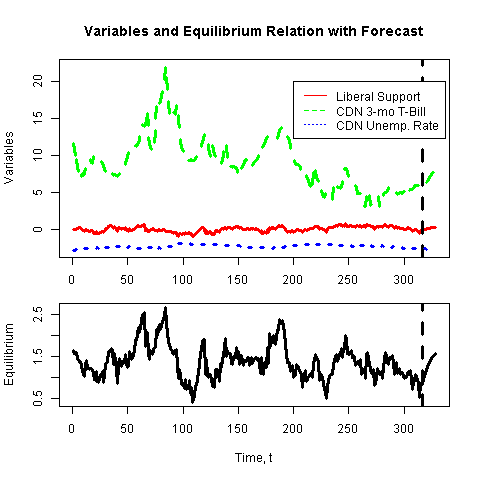
\includegraphics[scale = 1, keepaspectratio=true]{Figures/forecast_vars_eqbm.png}
  \caption{Forecast and equilibrium relationship of final model 12 steps ahead}
  \label{fig:forecast}
\end{figure}


The user specifies the forecast horizon (\verb|NumPeriods|) as well as the model (in this case, \verb|modelF <- m1r4|). These two inputs, along with the data, are used in the call to the function \fct{FCVARforecast}. This function returns \verb|xf|, a \verb|NumPeriods| by $p$ matrix of forecasted values of $X$, 
which are forecasted to take place after \verb|x1|. 
% This code section also plots the original series and the equilibrium relation $X\hat{\beta}$  along with the forecasts. These plots are shown in Figure~\ref{fig:forecast}.
Figure~\ref{fig:forecast} plots the original series and the equilibrium relation $X\hat{\beta}$, stored in \verb|equilF|,  along with the forecasts. 
% Figure~\ref{fig:forecast_vars} plots the original series and Figure~\ref{fig:forecast_eqbm} plots the equilibrium relation $X\hat{\beta}$, stored in \verb|equilF|,  along with the forecasts. 


%The forecasts can be printed to screen by typing \verb|xf| in the command window. For this example, the forecast yields the following output:
%\begin{verbatim}
%xf =
%
%   -0.143651232445609   5.857045691984009  -2.636093400885282
%   -0.084880236401301   5.959876423543075  -2.654427734412809
%   -0.025317647188555   6.110372247993035  -2.673504395263888
%    0.023637193159649   6.291703833118448  -2.692354312615941
%    0.065948385719753   6.495095415827381  -2.710793696483187
%    0.101480482760750   6.712274724017515  -2.728550463910498
%    0.131038772676406   6.937036380068601  -2.745463810349039
%    0.155108028894535   7.164423215402036  -2.761407736878001
%    0.174198620780072   7.390568568007144  -2.776296703046935
%    0.188773441631705   7.612444943293763  -2.790074682226306
%    0.199275426254352   7.827704702527144  -2.802710965769232
%    0.206124920473081   8.034550676278421  -2.814195673339702
%\end{verbatim}

%\begin{figure}[H]
%  \centering
%  % 
\includegraphics[scale = 1, keepaspectratio=true]{Figures/forecast.png}
%\subfigure{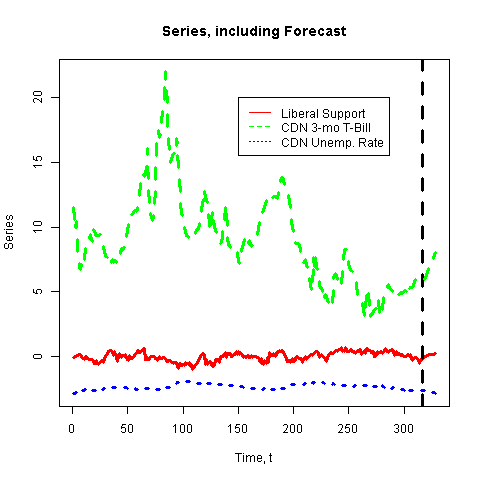
\includegraphics[scale = 1, keepaspectratio=true]{Figures/forecast_vars.png}}\\
%\subfigure{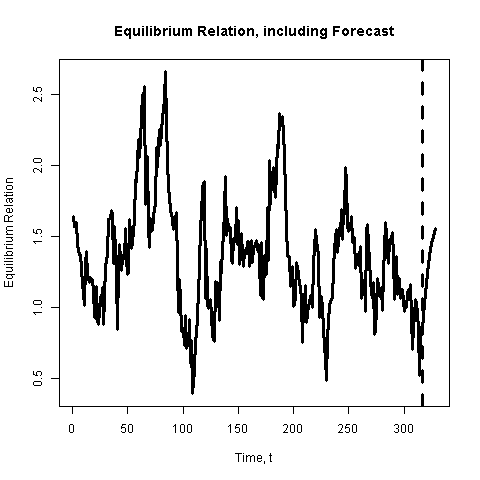
\includegraphics[scale = 1, keepaspectratio=true]{Figures/forecast_eqbm.png}}
%  \caption{Forecast of final model 12 steps ahead}
%  \label{fig:forecast}
%\end{figure}


%\begin{figure}[H]
%  \centering
%  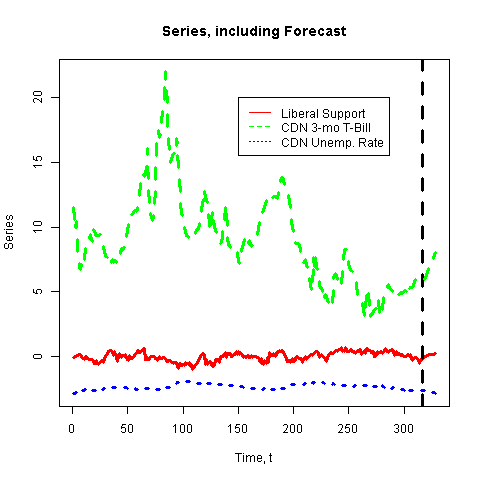
\includegraphics[scale = 1, keepaspectratio=true]{Figures/forecast_vars.png}
%  \caption{Forecast of final model 12 steps ahead}
%  \label{fig:forecast_vars}
%\end{figure}
%
%\begin{figure}[H]
%  \centering
%  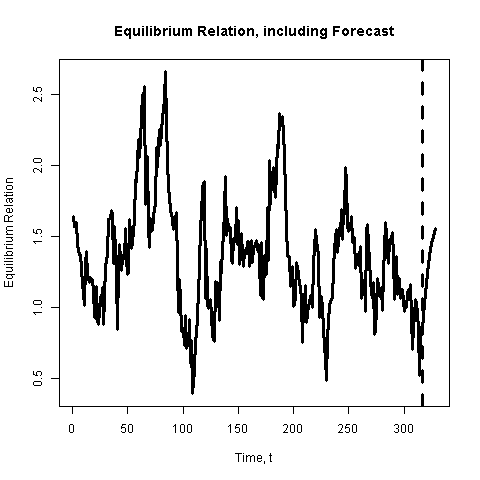
\includegraphics[scale = 1, keepaspectratio=true]{Figures/forecast_eqbm.png}
%  \caption{Forecast equilibrium relationship of final model 12 steps ahead}
%  \label{fig:forecast_eqbm}
%\end{figure}



\subsection{Bootstrap hypothesis test}
\label{sec:bootstr-hypoth-test}

% Listing~\ref{BSh} 
This code block
demonstrates the use of the wild bootstrap for hypothesis tests on the parameters, as developed by \cite{Boswijk2013} for the CVAR model. 
The function \fct{FCVARboot} returns the results of the wild bootstrap. 
The user specifies two sets of options corresponding to two different nested models, the restricted model with \verb|optRES| and the unrestricted model with \verb|optUNR|. 
This particlar example tests the restriction that political variables do not enter the cointegrating relation(s).

% The wild bootstrap is programmed to perform under parallel processing. If the user has the capability to use multiple processors, then computation time can be greatly reduced. 
% If not, the function can still be performed, but the bootstrap iterations will appear out of order since the loop is coded using \verb|parfor| instead of \verb|for|. 


%\begin{lstlisting}[frame=single,caption={Bootstrap hypothesis test}, label = BSh]
%% --------- BOOTSTRAP HYPOTHESIS TEST ---------- %
\begin{Code}
R> DefaultOpt$plotRoots <- 0
R> optUNR <- DefaultOpt
R> optRES <- DefaultOpt
R> optRES$R_Beta <- matrix(c(1, 0, 0), nrow = 1, ncol = 3)
R> set.seed(42)
R> FCVARboot_stats <- FCVARboot(x1, k, r, optRES, optUNR, B = 999)
R> LRbs_density <- density(FCVARboot_stats$LRbs)
\end{Code}

%% Plot bootstrap density with chi-squared density
%figure; plot(XI,F, XI, chi2pdf(XI,H.df))
%
%legend(['Bootstrap PDF with ', num2str(B), ' BS samples'],...
%    ['Chi Squared with ', num2str(H.df),' df'])
%\end{lstlisting}

An example of the output is
\begin{verbatim}
Bootstrap likelihood ratio test results:
Unrestricted log-likelihood: 451.174
Restricted log-likelihood:   444.395
Test results (df <- 1):
LR statistic: 	 13.557
P-value: 	 0.000
P-value (BS): 	 0.021
\end{verbatim}

The user might also be interested in comparing the bootstrap likelihood ratio test statistic distribution to the asymptotic one, a $\chi$-squared distribution with \verb|H$df| degrees of freedom. 
% The second part of Listing~\ref{BSh} performs this comparison by producing 
These objects can be used to produce 
a plot of the two distributions, shown in Figure~\ref{fig:BS}.

\begin{figure}[tbh]
  \centering
  
\includegraphics[scale = 1, keepaspectratio=true]{Figures/LRdensity_bw045.png}
  \caption{Density of bootstrap LR test statistic}
  \label{fig:BS}
\end{figure}


\subsection{Bootstrap rank test}
\label{sec:bootstrap-rank-test}

% Listing~\ref{BSr}
This code block
shows how to perform a wild bootstrap rank test, following the methodology of \cite{Cavaliere2010} for the CVAR model. This procedure works in much the same way as the bootstrap hypothesis test described in Section~\ref{sec:bootstr-hypoth-test}. The difference is that, instead of providing two sets of estimation options, the user specifies two different ranks for comparison.

%\begin{lstlisting}[frame=single,caption={Bootstrap rank test}, label = BSr]
%% --------- BOOTSTRAP RANK TEST ---------- %
% Test rank 0 against rank 1
\begin{Code}
R> r1 <- 0
R> r2 <- 1
R> FCVARbootRank_stats <- FCVARbootRank(x1, k, DefaultOpt, r1, r2, B = 999)
R> cat(sprintf('P-value: \t %1.3f\n', rankTestStats$pv[1]))
\end{Code}
% Compare to P-value based on asymptotic distribution
% fprintf('P-value: \t %1.3f\n', rankTestStats.pv(1));
%\end{lstlisting}

The results are printed as
\begin{verbatim}
Bootstrap rank test results:
Unrestricted log-likelihood: 451.174
Restricted log-likelihood:   440.040
Test results:
LR statistic: 	 22.268
P-value (BS): 	 0.031
# Need to modify program (with a particular seed):
P-value: 	 0.043
\end{verbatim}
in which the last $p$~value is printed to compare the bootstrap $p$~value to that based on the asymptotic distribution. 

\subsection{Simulation}
\label{sec:simulation}

Finally, 
% Listing~\ref{simFCVAR} 
this example
shows how to simulate an FCVAR model for a given set of parameters. The user provides data for starting values and a list containing model parameters for simulation as well as the number of periods to simulate. The simulated data are generated using Gaussian errors.

%\begin{lstlisting}[frame=single,caption={Simulation}, label = simFCVAR]
%% --------- SIMULATION ---------- %
\begin{Code}
R> T_sim <- 100
R> xSim <- FCVARsim(x1, modelF, T_sim)
\end{Code}
% Plot the results
%figure;
%plot(xSim)
%legend('Support', 'Unemployment', 'Interest rate')
%\end{lstlisting}

For the example above, 
using the same data as for the forecasting example above, 
the generated data is shown in Figure~\ref{fig:sim}.

\begin{figure}[tbh]
  \centering
  
\includegraphics[scale = 1, keepaspectratio=true]{Figures/sim.png}
  \caption{Simulated data}
  \label{fig:sim}
\end{figure}






%% -- Summary/conclusions/discussion -------------------------------------------

%% -- Extensions ---------------------------------------------------------------------

% \section{Extensions} \label{sec:extensions}

%\subsection{Extension for $p$~values} \label{sec:fdpval}
%
% Users don't need to do this in R:
% 
% We will simply mention it in the section on rank selection. 
%
%Although the MATLAB program can run standalone, one of the functions, \verb|FCVARrankTests.m|, makes an external system call to a separately installed program, \verb|fdpval|. This external program is the C++ implementation of a Fortran program used to obtain simulated $p$~values from \cite{mackinnon2014numerical}. If the user would like $p$~values for the cointegration rank tests to be automatically calculated, we recommend obtaining this companion program, which is made available by Jason Rhinelander and can be downloaded from: 
%\begin{center} \url{https://github.com/jagerman/fracdist/releases}
%\end{center}
%It can be either installed or downloaded in a compressed folder. It is important to note where the program is stored or installed, because the MATLAB program requires the program location as an input in the estimation options. For example, if the program is stored in the folder \verb|/usr/bin/| on a Linux system, the location variable is defined as follows, \verb|progLoc = '"/usr/bin/fdpval"'|. For details see Sections~\ref{sec:estoptions.m} and~\ref{sec:getpvals}.

% \subsection{Dealing with Local Optima}
\subsection{Plotting the likelihood function} \label{sec:extensions}



Users should be aware that the likelihood function is sometimes badly behaved, in that there may be local optima. To mitigate this problem...

We also make use of the excellent \verb|extrema.m| and \verb|extrema2.m| functions, which are written by Carlos Adrián Vargas Aguilera and are freely available from the Mathworks website. For simplicity these are included in the Auxiliary subfolder.

\begin{leftbar}
The above functions are currently not implemented in the R package, although I think there exist functions that already do this. 
Can we provide a use case in which the functions correct a problem or improve efficiency in the optimization?
The reason I ask is that I don't have a test case in which I needed to use this feature. 
\end{leftbar}

These functions are used in \fct{FCVARlikeGrid}, which allows the user to pre-estimate to obtain starting values by using a grid search. There are four types of estimation that the grid search can perform. If $d$ and $b$ are completely unconstrained, the grid search is over two dimensions within the bounds specified by \verb|opt$dbMin| and \verb|opt$dbMax|. An example of the likelihood obtained in an unconstrained grid search is shown in Figure~\ref{fig:gridFree}. Next, if $d\ge b$ is imposed via \verb|opt$constrained <- 1| (imposed in \cite{johansen2012likelihood} but relaxed in \cite{JN2018}) the computation can be cut in half. An example of this likelihood is shown in Figure~\ref{fig:gridConstrained}. If the restriction $d=b$ is imposed, then the grid search is one-dimensional as shown in Figure~\ref{fig:gridDB}. Finally, if a restriction is imposed on either $d$ or $b$ via $R_\psi$ and $r_\psi$ in \eqref{R psi}, then the grid search is also one-dimensional. An example of this situation is shown in Figure~\ref{fig:gridPhi}. Note that the $x$-axis is over the parameter $\phi$ and the fractional parameters are found from
\begin{equation}
  \begin{bmatrix}
    d \\ b
  \end{bmatrix}
  % [d \quad b]
  = H\phi + h,
\end{equation}
where $H = (R_{\psi}^{\prime})_\perp$ and $h = R_{\psi}^{\prime} (R_\psi R_{\psi}^{\prime})^{-1} r_\psi$. The bounds on $\phi$ are derived from \verb|opt$dbMin| and \verb|opt$dbMax| in a similar way\footnote{In this figure, the parameters are chosen so that $R_{\psi} = (2, -1)$ and $r_\psi$ = 0.5}.

% I have no idea why this wasn't as easy as it should have been:
\begin{figure}[H]
  \centering
  \subfigure[Unconstrained]{
    \label{fig:gridFree}
    % 
\includegraphics[scale = 0.10, keepaspectratio=true]{Figures/grid3d.png}
    
\includegraphics[width = 200pt]{Figures/grid3d.png}
  } 
  \subfigure[$d\ge b$]{ 
    \label{fig:gridConstrained}
    % 
\includegraphics[scale = 0.10, keepaspectratio=true]{Figures/gridConst.png}
    
\includegraphics[width = 200pt]{Figures/gridConst.png}
  }
  \\
  \subfigure[$d = b$]{
    \label{fig:gridDB}
    % 
\includegraphics[scale = 0.10, keepaspectratio=true]{Figures/gridDB.png}
    
\includegraphics[width = 200pt]{Figures/gridDB.png}
  } 
  \subfigure[Restrictions imposed]{
    \label{fig:gridPhi}
    % 
\includegraphics[scale = 0.10, keepaspectratio=true]{Figures/gridPhi.png}
    
\includegraphics[width = 200pt]{Figures/gridPhi.png}
  }
  \caption{Grid search}
  \label{fig:LikeGrid}
\end{figure}





%% -- Summary/conclusions/discussion -------------------------------------------

\section{Summary and discussion} \label{sec:summary}

\begin{leftbar}
Should we talk about anything in the pipeline, such as the stata version or the multifractional version?
I am leaning toward including the multifractional version on the repository in a development repo as a beta version. That way, it will be available to power users with the \pkg{devtools} package, where this version can be installed by 

\verb|devtools::install_github(LeeMorinUCF/FCVAR)|. 

In the meantime, we can run it through some tests and examples before putting it on the version in the repository. 
Anything else we want to include?
\end{leftbar}

%% -- Optional special unnumbered sections -------------------------------------

\section*{Computational details}

%\begin{leftbar}
%If necessary or useful, information about certain computational details
%such as version numbers, operating systems, or compilers could be included
%in an unnumbered section. Also, auxiliary packages (say, for visualizations,
%maps, tables, \dots) that are not cited in the main text can be credited here.
%\end{leftbar}

The results in this paper were obtained using
\proglang{R}~3.5.1. 
with the \pkg{FCVAR} package Version 0.0.0.9000. 
When determining cointegrating rank, the $p$~values for rank tests are obtained using the 
\pkg{fracdist} package Version 0.0.0.9000. 
\proglang{R} itself
and all packages used are available from the Comprehensive
\proglang{R} Archive Network (CRAN) at
\url{https://CRAN.R-project.org/}.

The latest version of the \proglang{MATLAB} package \pkg{FCVARmodel.m} in \cite{Nielsen2016} 
can be downloaded from one of the author's website at Queen's University:
% 
\begin{center} \url{http://www.econ.queensu.ca/faculty/mon/software/}
\end{center}
% 
\noindent It is freely available for non-commercial, academic use. 
The use of this program requires a functioning installation of MATLAB. 
The version of \proglang{MATLAB} available at the release of the last version was \proglang{MATLAB} 9.0, 	R2016a, number 35. However, any recent version should work.  
\proglang{MATLAB} users can simply unzip the contents of the zip file into any directory that they plan to use as the working directory of the program.



\section*{Acknowledgments}

%\begin{leftbar}
%All acknowledgments (note the AE spelling) should be collected in this
%unnumbered section before the references. It may contain the usual information
%about funding and feedback from colleagues/reviewers/etc. Furthermore,
%information such as relative contributions of the authors may be added here
%(if any).
%\end{leftbar}

We are grateful to Federico Carlini, Andreas Noack Jensen, S\o ren Johansen, Maggie Jones, James MacKinnon, Harry J. Paarsch, Jason Rhinelander, and Daniela Osterrieder for comments, and to the Canada Research Chairs program, the Social Sciences and Humanities Research Council of Canada (SSHRC), and the Center for Research in Econometric Analysis of Time Series (CREATES, funded by the Danish National Research Foundation DNRF78) for financial support.


%% -- Bibliography -------------------------------------------------------------
%% - References need to be provided in a .bib BibTeX database.
%% - All references should be made with \cite, \citet, \citep, \citealp etc.
%%   (and never hard-coded). See the FAQ for details.
%% - JSS-specific markup (\proglang, \pkg, \code) should be used in the .bib.
%% - Titles in the .bib should be in title case.
%% - DOIs should be included where available.

\bibliography{references}

%\begin{leftbar}
%Note that References have to be written in Title Case, as opposed to sentence case, 
%sometimes contrary to the convention in the journals themselves. 
%\end{leftbar}


%% -- Appendix (if any) --------------------------------------------------------
%% - After the bibliography with page break.
%% - With proper section titles and _not_ just "Appendix".

% \newpage

% \begin{appendix}

% \section{More technical details} \label{app:technical}

%\begin{leftbar}
%Appendices can be included after the bibliography (with a page break). Each
%section within the appendix should have a proper section title (rather than
%just \emph{Appendix}).
%
%For more technical style details, please check out JSS's style FAQ at
%\url{https://www.jstatsoft.org/pages/view/style#frequently-asked-questions}
%which includes the following topics:
%\begin{itemize}
%  \item Title vs.\ sentence case.
%  \item Graphics formatting.
%  \item Naming conventions.
%  \item Turning JSS manuscripts into \proglang{R} package vignettes.
%  \item Trouble shooting.
%  \item Many other potentially helpful details\dots
%\end{itemize}
%\end{leftbar}

% Technical details go here. 


%\section[Using BibTeX]{Using \textsc{Bib}{\TeX}} \label{app:bibtex}
%
%\begin{leftbar}
%References need to be provided in a \textsc{Bib}{\TeX} file (\code{.bib}). All
%references should be made with \verb|\cite|, \verb|\citet|, \verb|\citep|,
%\verb|\citealp| etc.\ (and never hard-coded). This commands yield different
%formats of author-year citations and allow to include additional details (e.g.,
%pages, chapters, \dots) in brackets. In case you are not familiar with these
%commands see the JSS style FAQ for details.
%
%Cleaning up \textsc{Bib}{\TeX} files is a somewhat tedious task -- especially
%when acquiring the entries automatically from mixed online sources. However,
%it is important that informations are complete and presented in a consistent
%style to avoid confusions. JSS requires the following format.
%\begin{itemize}
%  \item JSS-specific markup (\verb|\proglang|, \verb|\pkg|, \verb|\code|) should
%    be used in the references.
%  \item Titles should be in title case.
%  \item Journal titles should not be abbreviated and in title case.
%  \item DOIs should be included where available.
%  \item Software should be properly cited as well. For \proglang{R} packages
%    \code{citation("pkgname")} typically provides a good starting point.
%\end{itemize}
%\end{leftbar}

% \end{appendix}

%% -----------------------------------------------------------------------------


\end{document}
